%%%%%%%%%%%%%%%%%%%%%%%%%%%%%%%%%%%%%%%%%%%%%%%%%%%%
\documentclass[a4paper,fleqn,10pt,twocolumn]{SICE_ISCS}
%\usepackage{url}
\usepackage{ascmac}
\usepackage{amssymb}
%\usepackage{amsmath}
%\usepackage{hyperref}
%\usepackage{lmodern}
\usepackage{breqn}
\usepackage{bm}
\usepackage{comment}
\usepackage{pdfpages}
\usepackage{algorithm}
\usepackage{algorithmic}

\makeatletter
\@ifundefined{theorem}{%
  \newtheorem{theorem}{定理}
}{}
\@ifundefined{definition}{%
  \newtheorem{definition}{定義}
}{}
\makeatother

%\usepackage{HERE}
%\usepackage[version=3]{mhchem}%%化学式
%\usepackage{siunitx}
% 日本語サポートのためのパッケージ
\usepackage{CJKutf8}
\usepackage{otf}
\usepackage[dvipdfmx]{hyperref}
\usepackage{pxjahyper}
\usepackage{cite}
\usepackage{ulem} % 打ち消し線のためのパッケージ
\DeclareGraphicsExtensions{.eps,.pdf,.png,.jpg}
\newcommand{\Tabref}[1]{{Table~\ref{#1}}}
\newcommand{\Equref}[1]{Equation~(\ref{#1})}
\newcommand{\Figref}[1]{{Fig.~\ref{#1}}}
\newcommand{\blue}[1]{\textcolor{blue}{#1}}
\newcommand{\red}[1]{\textcolor{red}{#1}}
\title{単調環境における協調自己位置推定のためのCollaborative Stein Particle Filter}

\author{Tomoki Arita${}^{1\dagger}$ and Toru Namerikawa${}^{2}$}
% The dagger symbol indicates the presenter.
\speaker{Tomoki Arita}

\affils{${}^{1}$School of Integrated Design Engineering, Keio University, Kanagawa, Japan\\
	    ${}^{2}$Department of System Design Engineering, Keio University, Kanagawa, Japan\\
(Tel: +81-45-563-1151; E-mail: arita.tomoki@keio.jp, namerikawa@sd.keio.ac.jp)\\
}
\abstract{%
農地や森林などの単調で広大な屋外環境では、画像マッチングによるグローバル自己位置推定は、累積誤差や外れ値の影響により失敗することが多い。特に複数エージェントによる協調推定では、各エージェントの誤った状態推定が全エージェントに影響し、システム全体の誤った推定確率がエージェントごとの外れ値の割合に応じて指数関数的に増加する。本研究では、Stein Particle FilterとRelaxed ADMMを組み合わせることで、従来の画像特徴量のマッチングに位置情報による尤度を考慮しつつ、複数のエージェント間で推定状態を合意するフレームワークを提案する。提案手法は、特殊ユークリッド空間SE(d)上での確率分布の表現と操作、ADMMによる分散最適化、パーティクルベースの表現による不確実性の適切な取り扱いにより、複数エージェント間の合意制約と多峰性分布の扱いを同時に可能にし、従来手法では困難であった外れ値混在環境下での安定的な位置合意を実現する。2次元および3次元シミュレーションと実機実験結果から、提案手法が外れ値の割合が0.2程度の環境下でも安定した収束を達成し、分布近似と勾配情報を活用することで、既存手法よりもロバストかつ柔軟な自己位置推定が可能であることが示された。
}

\keywords{%
Collaborative Localization, Unmanned Aerial Vehicles, Stein Particle Filter, Monotone Environments, Visual-Inertial Navigation System.
}

\begin{document}

\maketitle

%-----------------------------------------------------------------------

\section{Introduction}
多くの自律移動可能なロボットは,動作の基盤となる自己位置推定を必要とする.また,自律移動ロボットの社会への浸透に伴って,過酷環境や山間地域等GPS/GNSSが利用できない環境での自己位置推定技術が数多く研究されている.自己位置推定には,力学制御や局所の動作計画などに利用する局所の自己位置推定の階層と,一貫した環境地図の作成や広域の経路計画に利用する大域の自己位置推定の階層が存在するが,GPS/GNSSが利用できない環境における大域の自己位置推定では,主にLiDARやカメラ等によって得られた点群及び画像データを種々のマッチング手法で構造化することにより自己位置推定を達成する手法が一般的である.実用的には,カメラとIMU(慣性計測ユニット)を組み合わせるVisual Inertial System(VINS)が安価にハードウェアを実装できる点から多く利用されている\cite{Qin2018}.

更に,自律移動ロボットの普及によって,複数のエージェントが同時に動作するマルチエージェント環境が近年主要な研究分野となっている.GPS/GNSSが使用できない過酷環境や山間地域においても,システム全体としての対故障性やそれぞれの目的におけるスケーラビリティの観点から,いくつかの研究でマルチエージェントによる協調作業が試みられている\cite{Chen2021}\cite{Zhou2018}.

これらの背景から,GPS/GNSSを用いない大域自己位置推定手法が求められているところであるが,農地や森林など単調かつ広大な野外環境下では,誤差の蓄積と外れ値の影響により画像のマッチングによる大域の自己位置推定が十分に機能しない.このような環境では,視覚的特徴の類似性や反復性により,特徴点マッチングに基づく従来のSLAM手法は誤対応を生じやすく,結果として位置推定の精度が著しく低下する.
特に複数のエージェントによる協調推定においては,各エージェントの誤った状態推定が全エージェントに影響する為,各エージェントの外れ値割合に伴ってシステム全体が誤った推定をする確率は指数関数的に上昇する.
そこで本研究では,確率分布の柔軟な表現が可能なStein Particle Filter(SPF)\cite{Liu2016}と分散最適化手法であるADMMを組み合わせることで,外れ値に対してロバストかつエージェント間で整合性のある協調自己位置推定フレームワークを提案する.本手法は,従来の画像特徴量マッチングに位置情報による尤度を統合し,多峰性分布の表現と複数エージェント間の状態合意を同時に実現する.
\begin{figure}[t]
	\begin{center}
		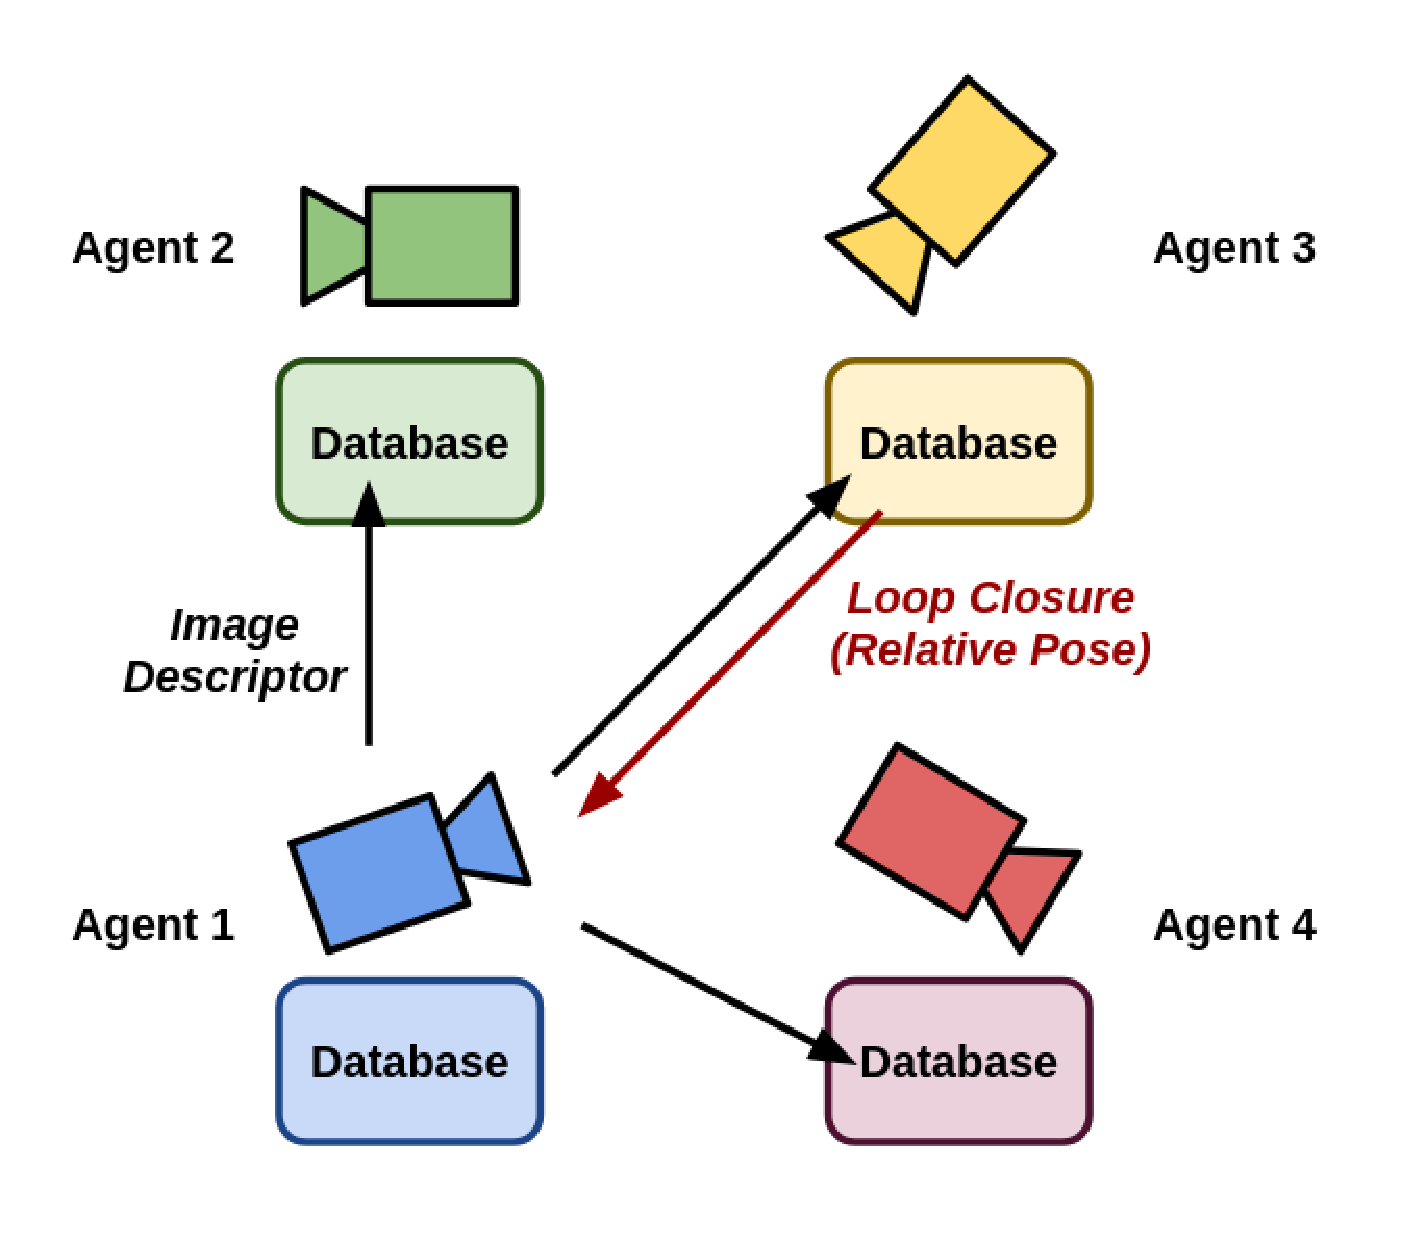
\includegraphics[width=\linewidth]{../Fig/simple_model.eps}
		\caption{Collaborative Visual Inertial Systemのモデル.通信時にagent1はagent3に画像特徴量データを送信し,agent3は送信されたデータを自信のデータベース内と照合してマッチングを行う.マッチングが検出されると,agent3は通信エッジを経由してagent1に相対位置に関するデータを送信する.}
		\label{fig:simple_model}
	\end{center}
	\vspace{-2mm}
\end{figure}

\subsection{Related Work}
本研究は,Visual Inertial Systems (VINS),マルチロボット協調SLAM,およびパーティクルフィルタと変分推論の分野に関連している.

VINSは,カメラとIMUを組み合わせて自己位置推定を行う手法であり,GPS/GNSSが利用できない環境で広く使用されている.Qinら\cite{Qin2018}は,単眼カメラとIMUを使用したロバストで汎用性の高いVINSであるVINS-Monoを提案し,特徴点追跡,IMU事前積分,ループ検出などの機能を統合した.Bloeschら\cite{Bloesch2017}は,直接的な光度フィードバックを用いた拡張カルマンフィルタベースのVINSを提案し,特徴点抽出に依存しない手法を実現した.Forsterら\cite{Forster2017}は,多様体上での事前積分を用いたリアルタイムVINSを提案し,IMU測定値を処理するための効率的な方法を示した.これらの研究は単一エージェントに焦点を当てており,複数エージェントの協調や単調環境の課題に十分に対応していない.

マルチロボット協調SLAMは,複数のロボットが協力して環境をマッピングし,位置を推定する方法である.Chenら\cite{Chen2021}は,データ融合の観点からマルチロボット協調SLAMの概要をまとめ,集中型,分散型,非集中型などの様々なアプローチを分類・比較した.Zhouら\cite{Zhou2018}は,実際の屋外環境におけるマイクロ空中ロボットの群れに関する研究を行い,協調自己位置推定の課題と解決策を示した.Xuら\cite{Xu2020}は,分散型の協調Visual-Inertial SLAMシステムであるD2SLAMを提案し,空中群れの効率的な協調自己位置推定を実現した.これらの研究は複数エージェントの協調に焦点を当てているが,単調環境における外れ値へのロバスト性や多峰性分布の処理に十分に対応していない.

パーティクルフィルタと変分推論は,非ガウス・非線形確率的状態推定問題を解くための手法である.LiuとWang\cite{Liu2016}は,本研究で使用するSPFの基礎となる一般的なベイズ推論アルゴリズムであるStein Variational Gradient Descent (SVGD)を提案した.Makenら\cite{Maken2021}は,非線形・非ガウス状態推定のためのSPFを提案し,従来のパーティクルフィルタにおけるリサンプリングによるパーティクル劣化の問題を解決した.Koideら\cite{Koide2021}は,GPUを用いたSPFの高速化に関する研究を行い,リアルタイムの6自由度位置推定を実現した.これらの研究はパーティクルフィルタと変分推論の理論と応用に焦点を当てているが,複数エージェントの協調やコンセンサス問題との組み合わせに十分に対応していない.

\subsection{Contributions}

本研究の主な貢献は以下の通りである.
\begin{itemize}
\item 2d及び3d上の協調自己位置推定を統一的に扱うため,特殊ユークリッド空間においてマルチエージェントに対するSPFを定式化した.これにより,visual inertial system等3次元の推定を必要とする実用的な協調自己位置推定に応用することが可能である.
\item ADMMの導入により,大域(複数エージェントでも一貫した)での収束が可能なSPFのアルゴリズムを提案した.これは従来の分散型協調推定手法では困難であった,エージェント間の一貫した状態推定を実現する.
\item 協調自己位置推定における曖昧性表現の獲得により,これまで単調環境において根本的な問題であった外れ値にロバストな推定手法を提案した.具体的には,多峰性分布の表現能力を持つパーティクルベース手法と勾配情報を活用したStein Variational Gradient Descentの組み合わせにより,外れ値の影響を局所化し,システム全体の推定精度を向上させた.
\end{itemize}

\section{Preliminary}

\subsection{Stein Variational Gradient Descent}
以下のようなカルバックライブラー情報量の最小化問題を考える.

\begin{equation}
\begin{aligned}\label{eq:kl_min}
 q^{*}&=\underset{q \in \mathcal{Q}}{\text{arg min}}\left\{D_{KL}(q \| p) \equiv {{\mathbb{E}}}_{q}[\log q(x)]-{{\mathbb{E}}}_{q}[\log {p}(x)] \right\},
\end{aligned}
\end{equation}

このとき以下の定理が成り立つ.

\begin{theorem}[KLダイバージェンスとStein Operatorの関係]
${\boldsymbol{T}}(x)=x+\epsilon {\boldsymbol{\Phi}}(x)$のような変換において,$x \sim q(x)$のとき$z={\boldsymbol{T}}(x)$の確率分布を$q_{[{\boldsymbol{T}}]}(z)$とすると
\begin{equation}
\begin{aligned}\label{eq:kl_gradient}
\left.\nabla_{\epsilon} D_{KL}\left(q_{[{\boldsymbol{T}}]} \| p\right)\right|_{\epsilon=0}=-{{\mathbb{E}}}_{x \sim q}\left[{\mathcal{A}}_{p} {\boldsymbol{\Phi}}(x)\right],
\end{aligned}
\end{equation}
が成り立つ.ただし${\mathcal{A}}_{p} {\boldsymbol{\Phi}}(x)=\nabla_{x} \log p(x) {\boldsymbol{\Phi}}(x)^{\top}+\nabla_{x} {\boldsymbol{\Phi}}(x)$はStein Operator, ${\boldsymbol{\Phi}}$は再生核ヒルベルト空間${\mathcal{H}}^d$に属する汎関数である.
\end{theorem}

ここで,Kernelized Stein Discrepancy(KSD)を

\begin{equation}
\begin{aligned}\label{eq:ksd}
{{\mathbb{D}}}(q,p)&=\max_{{\boldsymbol{\Phi}}\in {\mathcal{H}}^d}{{\mathbb{E}}}_{x \sim q}\left[{\mathcal{A}}_{p} {\boldsymbol{\Phi}}(x)\right], 
\quad \text{s.t.} \quad \|{\boldsymbol{\Phi}}\|_{{\mathcal{H}}^d} \leq 1,
\end{aligned}
\end{equation}

のように定義すると,この問題の解は

\begin{equation}
\begin{aligned}\label{eq:phi_solution}
{\boldsymbol{\Phi}}_{q, p}^{*}(\cdot)={{\mathbb{E}}}_{x \sim q}\left[k(x, \cdot) \nabla_{x} \log p(x)+\nabla_{x} k(x, \cdot)\right],
\end{aligned}
\end{equation}

で与えられる.

\subsection{Relaxed ADMM}

以下のような2変数に関する制約付き最適化問題

\begin{equation}
\begin{aligned}\label{eq:constrained_opt}
&\min_{x,y} f(x)+g(y), \quad \text{s.t.}\: Ax+By=b,
\end{aligned}
\end{equation}

は,次のような拡張ラグランジアン

\begin{equation}
\begin{aligned}\label{eq:augmented_lagrangian}
{\mathcal{ L}}_{f,\gamma}(z) &= f(x) - \langle z, Ax \rangle + \frac \gamma 2 \|Ax\|^2,\\
{\mathcal{ L}}_{g,\gamma}(z) &=  g(y) - \langle z, By-b \rangle + \frac \gamma 2 \|By-b\|^2,
\end{aligned}
\end{equation}

を用いて

\begin{equation}
\begin{aligned}\label{eq:relaxed_admm_steps}
y^+&= \underset{y}{\text{arg min}}\: {\mathcal{ L}}_{g,\gamma}(z),\\
\omega_g &=  z - \gamma (By^+-b), \\
x^+&= \underset{x}{\text{arg min}}\: {\mathcal{ L}}_{f,\gamma}(2\omega_g - z),\\
\omega_f &= 2\omega_g - z - \gamma Ax^+,\\
z^+&=z+\eta(\omega_f-\omega_g),
\end{aligned}
\end{equation}

の様な双対上昇法で解くことができる\cite{Peng2016}\cite{Boyd2011}.

\section{Problem Formulation}

本文では,ユークリッド空間${{\mathbb{R}}}^d$に存在するエージェントの協調自己位置推定を扱う.
時間ステップ$t$におけるエージェント$i$の状態を$x_i^t=({\mathbf{t}}^t_i, R^t_i)\in \mathrm{SE}(d):={{\mathbb{R}}}^d\times \mathrm{SO}(d)$,ここで座標${\mathbf{p}}^t_i\in{{\mathbb{R}}}^d$及び回転行列$R^t_i\in \mathrm{SO}(d)$である.また,手法の検証においては$d=2$, $d=3$の場合で検証を行う.協調自己位置推定は,各エージェントの観測を$z^t=[z_1^t, \cdots, z_N^t]$とすると,
以下のような最大事後確率推定問題(MAP推定問題)

\begin{equation}
\begin{aligned}\label{eq:map}
\underset{x^{t+1}_1, \cdots, x^{t+1}_N}{\text{max}} \: \sum^N_{i=1} P(x^{t+1}_i|Z_i^{t}) Q(z_i^{t+1}|x_i^{t+1}),
\end{aligned}
\end{equation}

として定式化できる.ここで,分布$P(x^{t+1}_i|Z_i^{t})$は時間ステップ$t+1$において,観測情報$z_i^{t+1}$が与えられる前のエージェント$i$の状態に関する確率分布を表し,分布$Q(z_i^{t+1}|x_i^{t+1})$は状態$x_i^{t+1}$において観測情報$z_i^{t+1}$が得られる尤度分布を表す.また,$Z_i^t = [z_i^0 \cdots z_i^t]$である.

3次元特殊ユークリッド群$\mathrm{SE(3)}$は以下の形式

\begin{equation}
\begin{aligned}\label{eq:se3_matrix}
T = 
\begin{pmatrix}
{\mathbf{R}} & {\mathbf{t}} \\
{\mathbf{0}}^T & 1
\end{pmatrix}
=
\begin{pmatrix}
{\mathbf{d}}_{c1} & {\mathbf{d}}_{c2} & {\mathbf{d}}_{c3} & {\mathbf{t}} \\
0 & 0 & 0 & 1
\end{pmatrix} \in {{\mathbb{R}}}^{4\times4},
\end{aligned}
\end{equation}

で表現される.ここで,特殊直交群$\mathrm{SO(d)}$及び特殊ユークリッド群$\mathrm{SE(d)}$における以下の演算子を導入する.

\begin{equation}
\begin{aligned}
(\cdot)^{\wedge}&: {{\mathbb{R}}}^{\frac{d(d-1)}{2}} \rightarrow  {\mathfrak{so}}(d), {{\mathbb{R}}}^{d+\frac{d(d-1)}{2}} \rightarrow  {\mathfrak{se}}(d),\\
{\boldsymbol{\omega}}&=\begin{bmatrix}
    \:x\: \\
    \:y\: \\
    \:z\: 
\end{bmatrix}\in{{\mathbb{R}}}^3,
\quad {\boldsymbol{\omega}}^{\wedge}=\begin{pmatrix}
    0&-z&y \\
    z&0&x \\
    -y&x&0 
\end{pmatrix}\in {\mathfrak{so}}(3)\\
{\mathbf{v}}&=\begin{bmatrix}
    \:{\mathbf{t}}\: \\
    \:{\boldsymbol{\omega}}\: 
\end{bmatrix}\in{{\mathbb{R}}}^6,\quad {\mathbf{v}}^\wedge=\begin{pmatrix}
    {{\boldsymbol{\omega}}^\wedge}& {\mathbf{t}}\\
    0&1
\end{pmatrix}\in {\mathfrak{se}}(3)
\end{aligned}
\end{equation}

\begin{equation}
\begin{aligned}
\exp&:  {\mathfrak{so}}(d) \rightarrow  \text{SO}(d),{\mathfrak{se}}(d) \rightarrow  \text{SE}(d),\\
\quad e^{{\boldsymbol{\omega}}} &\equiv \exp({{\boldsymbol{\omega}}}^\wedge) \\
&= {\mathbf{I}}_3 + \frac{\sin \theta}{\theta } {{\boldsymbol{\omega}}}^\wedge+\frac{1-\cos \theta }{\theta^2}({{\boldsymbol{\omega}}}^\wedge)^2 \in \text{SO}(3)\\
e^{{\mathbf{v}}}&\equiv \exp({{\mathbf{v}}^\wedge}) = 
\begin{pmatrix}
    e^{{{\boldsymbol{\omega}}}^\wedge}& {\mathbf{V}}{\mathbf{t}}\\
    0&1
\end{pmatrix}\in\text{SE}(3),\quad \\
{\mathbf{V}}&={\mathbf{I}}_3+\frac{1-\cos\theta}{\theta^2}{{\boldsymbol{\omega}}}^\wedge +\frac{\theta-\sin \theta}{\theta^3}({{\boldsymbol{\omega}}}^\wedge)^2
\end{aligned}
\end{equation}

更に,$()^\vee$,$\log$はそれぞれ$()^\wedge$,$\exp$の逆演算を表す.
SPFにおける一般的な手法として,式(\ref{eq:map})をカルバック・ライブラー情報量(KLダイバージェンス)$D_{KL}$の最小化問題

\begin{equation}
\begin{aligned}
  &\underset{x_i^{t+1}}{\text{max}} \:  P(x_i^{t+1}|Z_i^{t}) Q(z_i^{t+1}|x_i^{t+1})\\
  &\simeq \underset{x_i^{t+1}}{\text{max}} \: \underset{P_{[T]}}{\text{arg min}} \: D_{KL}(P(x_i^{t+1}|Z_i^{t})_{[T]} \| P_Q),
\end{aligned}
\end{equation}

に置き換える.ここで目標分布$P_Q$は尤度分布$Q$と同型の状態$x_i^{t+1}$についての確率分布であり,平均座標$\mu\in\mathrm{SE}(d)$及び重み対角行列$\Sigma \in {{\mathbb{R}}}^{(d+\frac{d(d-1)}{2})\times (d+\frac{d(d-1)}{d})}$を用いて,$\mathrm{SE(3)}$上におけるカーネル

\begin{equation}
\begin{aligned}
{\mathcal{K}}_j&=\exp \left(-(d_j^\vee)^{\top} \Sigma d_j^\vee \right)\in {{\mathbb{R}}},\\
d_j&=\log \left((\mu_j^{-1}) x_i^{t+1} \right)\in {\mathfrak{se}}(d)
\end{aligned}
\end{equation}

の重ね合わせで表現される.これらの背景から,時間ステップtにおいてエージェントiからみたエージェントjの状態$x_{i,j}^t$をとし,推定する状態量を$\hat x_i^t= \left\{ x_{i,j}^t \in \mathrm{SE(d)}\: | \: j \in \mathcal{N}_i \right\}$のように修正することで解くべき問題は
\begin{equation}
\begin{aligned}\label{eq:kl_consensus}
\max _{\hat x_{1}^{t}, \cdots, \hat x_{N}^{t}} & \sum_{i=1}^{N} \arg \min _{{P_{i}}_{[T]}} D_{K L}\left(P_{i}\left(\hat x_{i}^{t} \mid Z_{i}^{t-1}\right)_{\left[T_{i}]\right.} \| P_{Q_{i}} \right) \\
\text { s.t. } & \hat x_{i}^{t}=\hat x_{j}^{t}, \quad\forall(i, j) \in \mathcal{E}
\end{aligned}
\end{equation}
のように定式化できる.この式(\ref{eq:kl_consensus})における制約は,エージェント間の通信を示すすべてのエッジ$\mathcal{E}$において,ドローンの推定状態が一致していることを示す.

\section{SPF For Collaborative Localization}

このセクションでは,式(\ref{eq:kl_consensus})の解を求めるためのSPFを用いた数学的アルゴリズムを提案する.確率分布におけるKLダイバージェンスの最小化は,SPFを用いることで数値計算可能である.一方で,マルチエージェント問題におけるKLダイバージェンスの最小化は絶対座標に固定された目標分布が存在せず,目標分布$P_{Q_i}$自体が推定したい状態量の従属変数となってしまうため非常に困難である.更に,式(\ref{eq:kl_consensus})のような制約の無い安易なSPFアルゴリズムを適用した場合,フィルタリングアルゴリズムは部分的な状態量に対してPartialにのみ最適化されるため,
後述するように,エージェント全体で統一された相対位置のグラフを作ることができず推定が破綻する.これらの問題を解決するため,我々は明示的なパーティクル間の相対位置を用いた尤度関数,およびRelaxed ADMMによる合意アルゴリズムを用いることでCollaborative Localizationに適用可能なSPFアルゴリズムを定式化した.

\subsection{パーティクル同士の勾配効果}

まず,確率分布を$P_{i}\left( x_{i}^{t} \mid Z_{i}^{t-1}\right)\simeq \left\{ p_{i,l}\in \mathrm{SE(3)} \right\}_{l=1:m}$のようにパーティクルで近似し,これらを式(\ref{eq:kl_consensus})に基づき目標分布$P_{Q_i}$にそって勾配降下させることを考える.

\begin{equation}
\begin{aligned}\label{eq:svgd_min}
&\underset{P_{[T]}}{\text{min}} \: \nabla_\epsilon \left . D_{KL}(P(x_i^{t+1}|Z^{t})_{[T]} \| P_{Q_i})\right |_{\epsilon = 0},\\
&\Rightarrow p_{i,l}:= p_{i,l} \exp({\boldsymbol{\Phi}}^*),\\
&\quad \:\: {\boldsymbol{\Phi}}^*(p_{i,l}) = \frac{1}{m}\sum_{r=1}^m(\nabla_{p_{i,r}}\log P_Q(p_{i,r})k(p_{i,l},p_{i,r}) \\
&\qquad \qquad \quad \: + \nabla_{p_{i,j}}k(p_{i,l},p_{i,r})),
\end{aligned}
\end{equation}
ここで$k(p_{i,l},p_{i,r})=\exp \left(-(d_j^\vee)^{\top} \Sigma d_j^\vee \right)\in \mathbb{R}$は$\mathrm{SE(3)}$上のカーネルである.

\begin{equation}
\begin{aligned}\label{eq:log_target_dist}
    \log P_{Q_i}(p_{i,r}) &= \log \prod_{k\in {\mathcal{N}}} {\mathcal{K}}_k\\
    &= -\sum_{k\in {\mathcal{N}}} (d_k^\vee)^{\top} \Sigma_k d_k^\vee \in \mathbb{R},\\
d_k(p_{i,r})&=\log \left(p_{j,k}^{-1} (p_{i,r}T_{i\rightarrow j}) \right)\in {\mathfrak{se}}(d)
\end{aligned}
\end{equation}

ここで$k\in{\mathcal{N}} := {\mathcal{N}}_{j}(p_{i,l}T_{i\rightarrow j})$であり,エージェントjが持つパーティクルの内,$T_{i\rightarrow j}\in \mathrm{SE(3)}$で変換したエージェントiが持つr番目のパーティクル$p_{i,r}$にとって近傍のパーティクルの集合を表す.このように得られた相対位置$T_{i\rightarrow j}$にそってパーティクルを変換した場合の予測位置近傍のパーティクルについて明示的に$\mathrm{SE(3)}$上の誤差を計算し,近傍でKDEにより真の目標分布を推定することで,固定された目標分布が存在しない場合においてもKLダイバージェンスを最小化することが可能である.
更に収束を高速化させるため,目標分布の勾配$\nabla_{p_{i,r}}\log P_Q(p_{i,r})$はガウスニュートン法を用いて
\begin{equation}
% \begin{equation}
\begin{aligned}\label{eq:gauss_newton}
\nabla_{p_{i,r}}\log P_Q(p_{i,r})&:=
({\mathbf{H}}^r)^{-1}b^r,\\
{\mathbf{H}}^r &= ({\mathbf{J}}^r)^\top {\mathbf{J}}^r, \\
b^r&=({\mathbf{J}}^r)^\top d_k(p_{i,r})^\vee,\\
{\mathbf{J}}^r&=\left. \frac{\partial(d_k(p_{i,r}e^{{{\boldsymbol{\varepsilon}}}})^\vee
)}{\partial {{\boldsymbol{\varepsilon}}}}\right|_{{{\boldsymbol{\varepsilon}}}={\mathbf{0}}}
\end{aligned}
% \end{equation}
\end{equation}
の様に計算を行う.

\subsection{SPF integrating Relaxed ADMM}

このサブセクションでは,サブセクションAで定式化したSPFによる勾配降下法をもとに,式(\ref{eq:kl_consensus})の合意制約付きKLダイバージェンスの最小化を行うアルゴリズムの定式化を行う.まず,単純(straightforward)な解法として
\begin{equation}
\begin{aligned}
&\underset{P_{[T]}}{\text{min}} \: \nabla_\epsilon \left . D_{KL}(P(x_i^{t+1}|Z^{t})_{[T]} \| P_{Q_i})\right |_{\epsilon = 0}, \quad 
\forall i\in \mathcal{A}
\end{aligned}
\end{equation}
のように,すべてのエージェントが相対位置を受け取った時点で各エージェントペアに対し相対位置パーティクルの更新を行う場合を考える.この場合,相対位置の送り元であるエージェントがグローバルに正しい位置に収束している保証が無いため,Fig. \ref{fig:parallel_update}(a)に示すように特定のエージェントペアでのみ最適化された位置関係に収束してしまい,エージェント全体で一貫した相対位置のグラフを構築することができない.フィルタリングによる種々の最適化は,複数の状態量を同時に最適化することができず,単一の状態量をpartialに最適化する必要がある.ここで,本手法では,Fig. \ref{fig:parallel_update}(b)のようにADMMによるconsensus filterを用いることで相対位置を取得できる順番に関わらず大域での収束を可能にするアルゴリズムを定式化する.

\begin{figure}[t]
	\begin{center}
		\includegraphics[width=\linewidth]{Fig/parallel_update1.eps}
		\caption{Fig. \ref{fig:simple_model}のようなシステムにおいて,各エージェントが相対位置を受けとり推定状態を並列に更新するシーケンス図.(a)は合意則を用いないstoraightforwardな方法,(b)は合意則を用いることにより大域での収束を可能にする手法}
		\label{fig:parallel_update}
	\end{center}
	\vspace{-2mm}
\end{figure}

式(\ref{eq:kl_consensus})はスラック変数$y_{i,j}$を用いて
\begin{equation}
\begin{aligned}
\max _{\hat x_{1}^{t}, \cdots, \hat x_{N}^{t}} & \sum_{i=1}^{N} \arg \min _{{P_{i}}_{[T]}} D_{K L}\left(P_{i}\left(\hat x_{i}^{t} \mid Z_{i}^{t-1}\right)_{\left[T_{i}]\right.} \| P_{Q_{i}} \right) \\
\text { s.t. } & \hat x_{i}^{t}=y_{i,j}, \:\hat x_{j}^{t}=y_{i,j}, \quad\forall(i, j) \in \mathcal{E}
\label{eq:kl_consensus_relaxed}
\end{aligned}
\end{equation}
のように緩和することにより,式(7)の問題に帰着できる.

\begin{definition}[確率分布に対する拡張ラグランジアン]
ここで,Relaxed ADMMにおける拡張ラグランジアンとして,確率分布を引数にもつ拡張ラグランジアンを
\begin{equation}
\begin{aligned}
 {\mathcal{ L}}_{F,\gamma}(x_i, \zeta) 
 = F_i(x_i) - \int_{{\mathcal{X}}_i}
\zeta dx_i + \frac{\gamma}{2}\int_{{\mathcal{X}}_i} dx_i^2,
\label{eq:relaxed_lagrangian}
\end{aligned}
\end{equation}
のように再定義する.
\end{definition}

これにより式(\ref{eq:kl_consensus_relaxed})は以下のアルゴリズム
以下に,式(\ref{eq:kl_consensus_relaxed})を解くための確率分布に対するRelaxed ADMMアルゴリズムを定理として示す.

\begin{theorem}[確率分布に対するRelaxed ADMMアルゴリズム]
式(\ref{eq:kl_consensus_relaxed})で表される確率分布に対する制約付き最適化問題は,以下のRelaxed ADMMアルゴリズムによって解くことができる:
\begin{equation}
\begin{aligned}
x^+_i&= \underset{x_i}{\text{arg min}}\: D_{KL} ({P_i}_{[T]}\|{P_Q}_i) \\
&+ \sum_{r\in {\mathcal{E}}_i} \int_{P_i}  z_{ir,r} dx_i + \frac{\gamma}{2}|{\mathcal{E}}_i|\int_{P_i} dx_i^2,\\
&= \underset{x_i}{\text{arg min}}\: D_{KL} ({P_i}_{[T]}\|{P_Q}_i) \\
&+ \frac{\gamma}{2} \:{\mathbb{E}}_{x_i\sim P_i}\left[\sum_{\gamma \in {\mathcal{E}}_i} \|x_i + z^+_{ir,i}/\gamma \|^2\right],\\
z^+_{ir,i} &=z_{ir,i}+\eta((z_{ir,i} + z_{ir,r})/2 + \gamma x_{i}).\quad  \forall r \in {\mathcal{E}}_i,
\label{eq:prob_relaxed_admm}
\end{aligned}
\end{equation}
ここで,$x^+_i$は更新後の状態,$z_{ir,i}$はラグランジュ乗数,$\gamma$はペナルティパラメータ,$\eta$はステップサイズパラメータである.このアルゴリズムは,各エージェントの局所的な確率分布の更新と,エージェント間の合意制約の両方を同時に最適化する.
\end{theorem}

このアルゴリズムにより,複数エージェント間の合意制約と確率分布の最適化を同時に行うことが可能となり,外れ値が存在する環境下でも安定した状態推定を実現できる.

\begin{theorem}[指数的なペナルティとしての追加項]
以下の最適化問題
\begin{equation}
\begin{aligned}
&\min_{P_i}  D_{KL}(P_i \,\|\, P_{Q_i}) \\
&+ \sum_{r \in {\mathcal{E}}_i} \int P_i(x_i) z_{ir,r}(x_i)\,dx_i 
+ \frac{\gamma}{2}|{\mathcal{E}}_i| \int P_i(x_i) x_i^2\, dx_i
\end{aligned}
\end{equation}
を考える.ただし,$\int P_i(x_i)dx_i=1$ であり,$D_{KL}(P_i \,\|\, P_{Q_i})$ は
\begin{equation}
\begin{aligned}
&\underset{x_i^{t+1}}{\text{max}} \:  P(x_i^{t+1}|Z_i^{t}) Q(z_i^{t+1}|x_i^{t+1})\\
&\simeq \underset{x_i^{t+1}}{\text{max}} \: \underset{P_{[T]}}{\text{arg min}} \: D_{KL}(P(x_i^{t+1}|Z_i^{t})_{[T]} \| P_Q),
\end{aligned}
\end{equation}
で定義される.このとき,上記の最適化問題に対する最適分布 $P_i^*$ は,ある正規化定数 $Z$ を用いて
\begin{equation}
\begin{aligned}
P_i^*(x_i) = \frac{P_{Q_i}(x_i)\exp\left(- \sum_{r \in {\mathcal{E}}_i} z_{ir,r}(x_i) 
- \frac{\gamma}{2}|{\mathcal{E}}_i| x_i^2\right)}{Z},
\end{aligned}
\end{equation}
と表せる.すなわち,追加のペナルティ項
\begin{equation}
\begin{aligned}
\sum_{r \in {\mathcal{E}}_i} z_{ir,r}(x_i) \;+\; \frac{\gamma}{2}|{\mathcal{E}}_i|x_i^2,
\end{aligned}
\end{equation}
は,基準分布 $P_{Q_i}(x_i)$ に対して指数的な重み(ペナルティ)を掛ける形で最適解を特徴づける.
\end{theorem}

したがって式(\ref{eq:prob_relaxed_admm})から,パーティクルの更新則は
\begin{equation}
\begin{aligned}
&\underset{x_i}{\text{min}}\: D_{KL} ({P_i}_{[T]}\|{P_Q}_i) \\
&\quad \:\: + \sum_{r\in {\mathcal{E}}_i} \int_{P_i} z_{ir,r} dx_i + \frac{\gamma}{2}|{\mathcal{E}}_i|\int_{P_i} dx_i^2,\\
&\Rightarrow p_{i,l}:= p_{i,l} \exp({\boldsymbol{\Phi}}^*),\\
&\quad \:\: {\boldsymbol{\Phi}}^*(p_{i,l}) = \frac{1}{m}\sum_{r=1}^m(\nabla_{p_{i,r}}\log {{P}^*_i}(p_{i,r})k(p_{i,l},p_{i,r}) \\
&\qquad \qquad \quad \: + \nabla_{p_{i,j}}k(p_{i,l},p_{i,r})),\\
&\quad \:\:  {{P}^*_i}(p_{i,r}) \propto {P}_{Q_i}(p_{i,r})\exp\left(- \sum_{r \in  {\mathcal{E}}_i} z_{ir,r}(p_{i,l}) - \frac{\gamma}{2}|{\mathcal{E}}_i| p_{i,l}^2\right),
\label{eq:modified_SVGD}
\end{aligned} 
\end{equation}

のように修正できる.これらの定式化により,式(\ref{eq:map})を解くためのアルゴリズムは以下のように表すことができる.

\begin{algorithm}[h]
\caption{SPF For Collaborative Localization}\label{alg:dspf}

\begin{algorithmic}[1]
\STATE \textbf{Input:} $n$ UAVs, $m$ particles $\{x^t_{i,j}\}^m_{j=1}$, Target distribution ${P_Q}_i$

\FOR{$k = 1$ to $K$}
\STATE preintegration by (\ref{eq:predict})
\ENDFOR
\STATE $\forall_{j=1:m}\; p^{t+1}_{i,j} = p^{t}_{i,j} T^{t \rightarrow {t+1}}$  // prediction (\ref{eq:step})
\FOR{$l = 1$ to $L$}
\STATE $\forall_{j=1:m}\;$ update particle by (\ref{eq:modified_SVGD})
\STATE $x_i = \underset{x_i}{\text{arg min}}\: {P_i(x_i)}$ // local MAP estimation
\STATE consensus update by (\ref{eq:prob_relaxed_admm})
\ENDFOR
\end{algorithmic}
\end{algorithm}

\section{Simulation Result with Collaborative Localization}

提案したアルゴリズムに基づき,2次元と3次元の場合において協調自己位置推定のシミュレーションを行った.アルゴリズムの実装においては,計算負荷の削減のため,全アルゴリズムをCUDA上に実装し,各パーティクルの更新をGPUで並列処理してシミュレーションを行った.Gauss Newton 法の求解にはcuSolverを用いた.ハードウェアはintel core ultra 9, NVIDIA GeForce RTX 4060を搭載したpcを用いた.

\subsection{Two-dimensional case}

提案手法の検証として,2Dにおける協調自己位置推定シナリオのシミュレーションを行った.シミュレーション条件を表\ref{tb:sim1}に示す.

\begin{table}[h]
\caption{シミュレーション条件}
  \centering
  \begin{tabular}{l|c} \hline
    項目 & 値  \\ \hline
    エージェント数 & 3  \\
    エージェントごとのパーティクル数 & 50  \\ 
    時間ステップ数 & 250 \\
    総マッチング数 & 250 \\ 
    誤マッチング数 & 52 \\
    外れ値の割合 & $\simeq$ 0.2 \\ \hline
  \end{tabular}
  \label{tb:sim1}
\end{table}

シミュレーションでは,各ステップランダムなエージェントペアの相対位置(擬似的なクロージャーループ, Fig. \ref{fig:simulation_1_step_0}内黒点線)がそれぞれ得られると仮定し,その相対情報を用いて各エージェントの位置を推定する.
また,約0.2の割合で誤った相対位置(Fig. \ref{fig:simulation_1_step_0}内赤点線)が得られると仮定し,matplotlibを用いて協調自己位置推定シミュレーションを行った.
Fig. \ref{fig:simulation_1_step_0}(a)左図が真の各エージェント位置,\ref{fig:simulation_1_step_0}(a)右図が推定画面である.
誤った相対位置は,シミュレーション領域内のランダムな座標と各エージェントの真の位置から生成した.

Fig. \ref{fig:simulation_1_step_0}(a), (b)はそれぞれ0ステップと150ステップにおける各エージェントの推定状態の様子である.
これらから,0ステップにおいては一様に設定されていた確率分布(パーティクル)が,150ステップにおいては妥当な位置に収束していることが分かる.
また,Fig. \ref{fig:plot_1}はシミュレーションにおける全パーティクルの座標の時間遷移である.
Fig. \ref{fig:plot_1}からも,150ステップほどで合意及び収束が達成されていることが分かる.

\begin{figure}[t]
	\begin{center}
		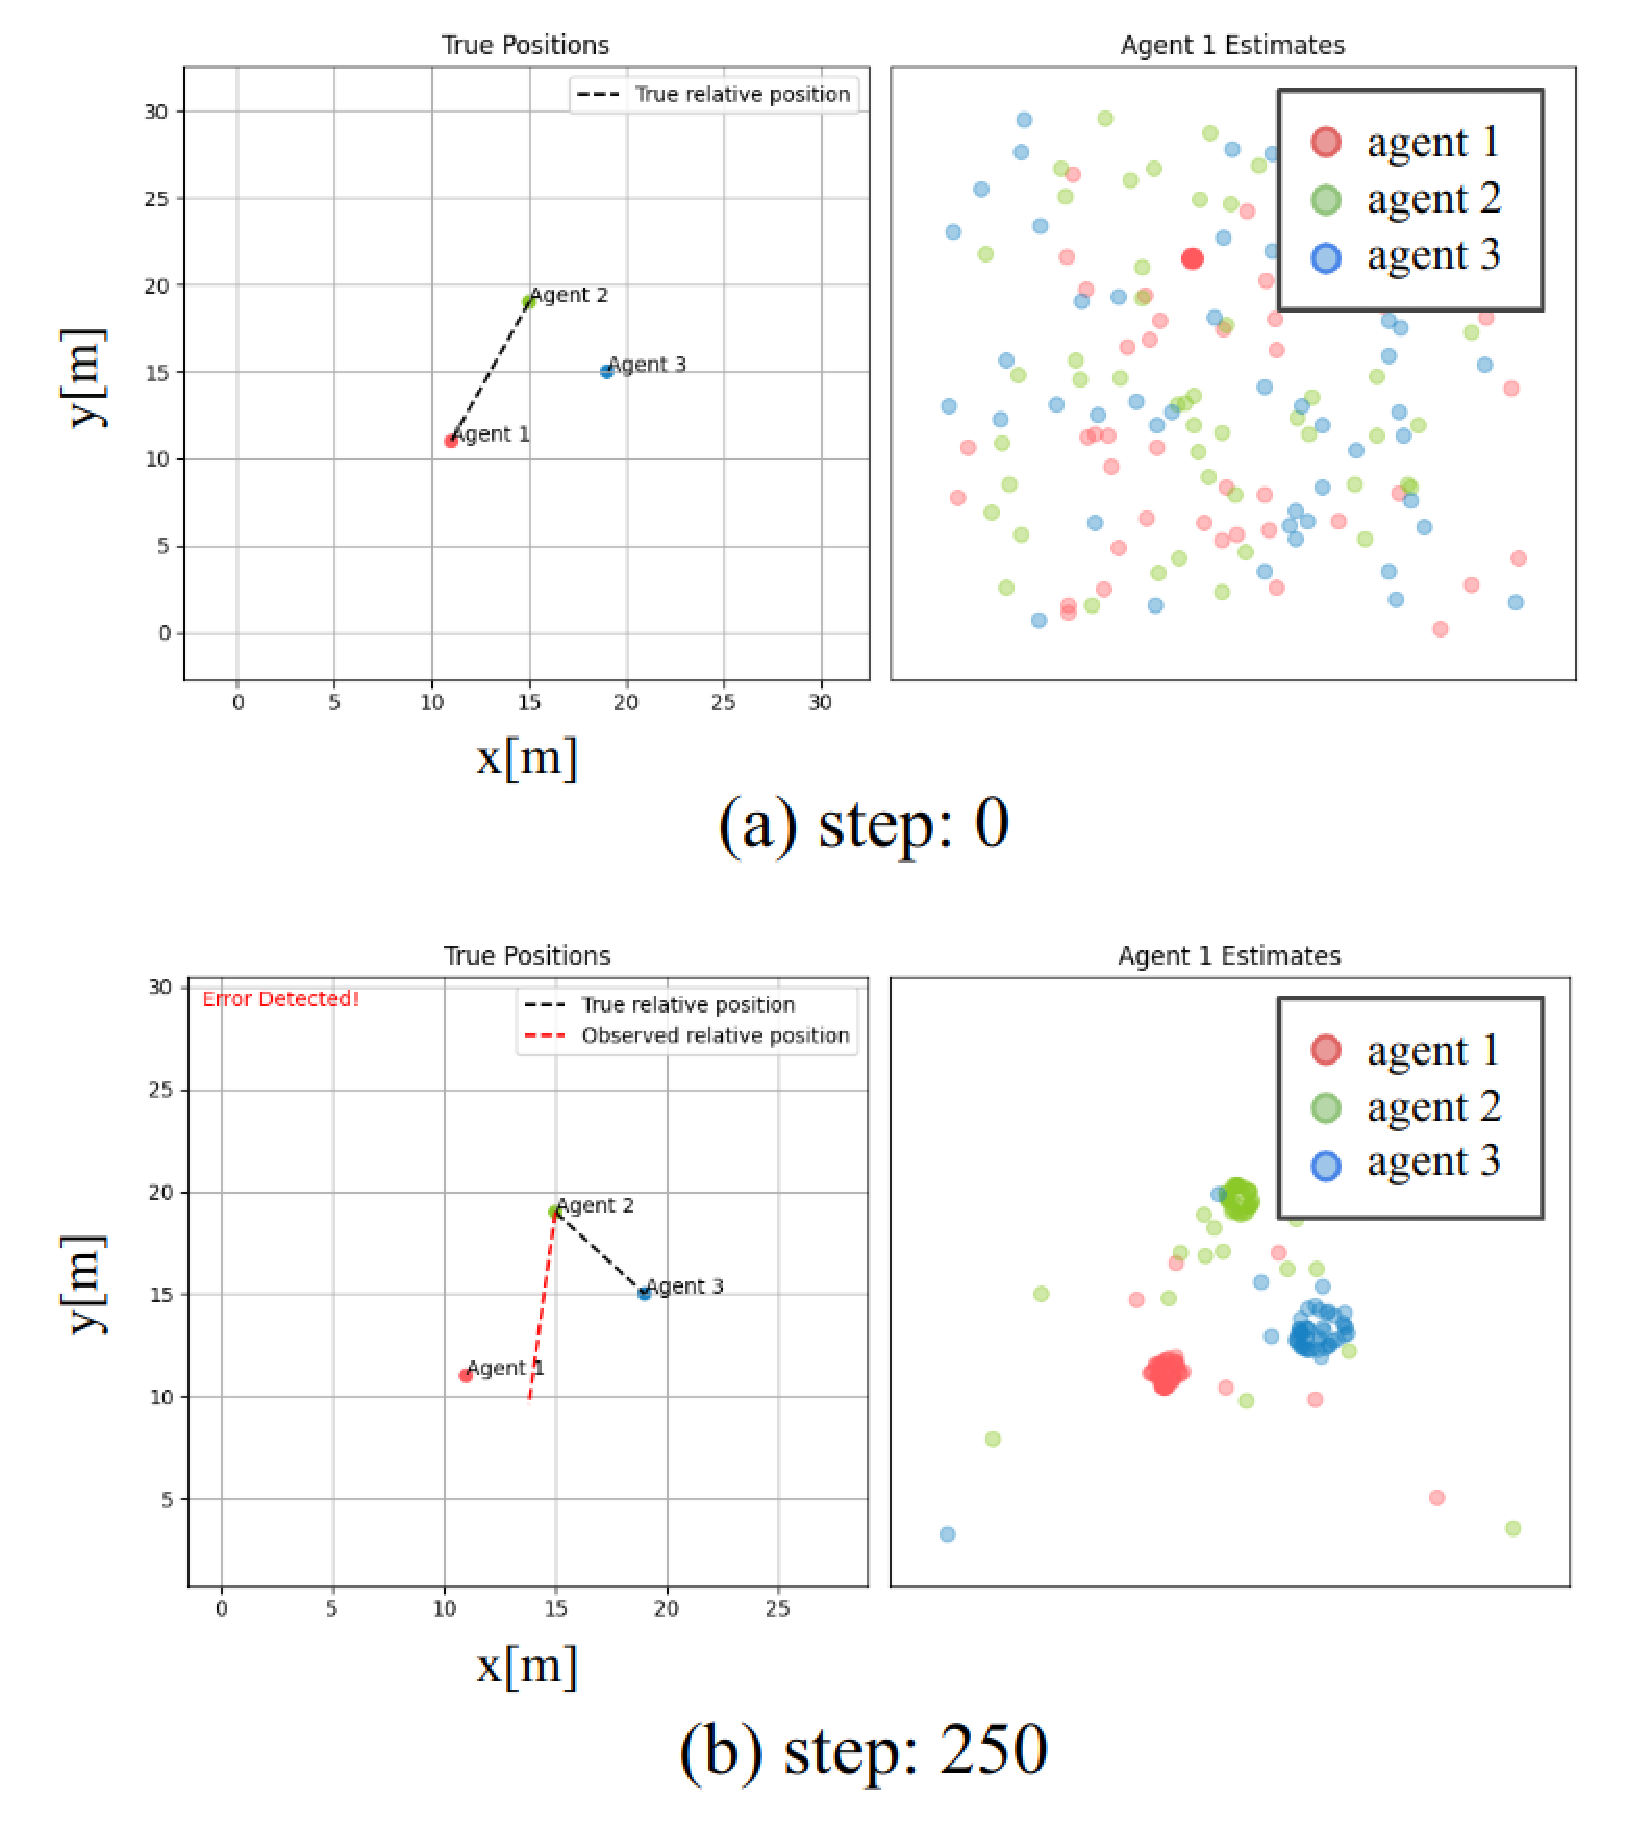
\includegraphics[width=\linewidth]{Fig/2d_simulation.eps}
		\caption{外れ値の割合が0.2の場合における,2次元の協調自己位置推定シミュレーション.(a)は初期状態,(b)は150ステップ目の様子.
    左図は各エージェントの真の位置,右図の点はそれぞれのエージェントにおけるパーティクルの座標$p_{i,r}$である.}
		\label{fig:simulation_1_step_0}
	\end{center}
	\vspace{-2mm}
\end{figure}

% \begin{figure}[t]
% 	\begin{center}
% 		\includegraphics[width=\linewidth]{Fig/error_0.2_sim.eps}
% 		\caption{シミュレーション (外れ値の割合:0.2, step: 150)}
% 		\label{fig:simulation_1_step_150}
% 	\end{center}
% 	\vspace{-2mm}
% \end{figure}

\begin{figure}[t]
	\begin{center}
		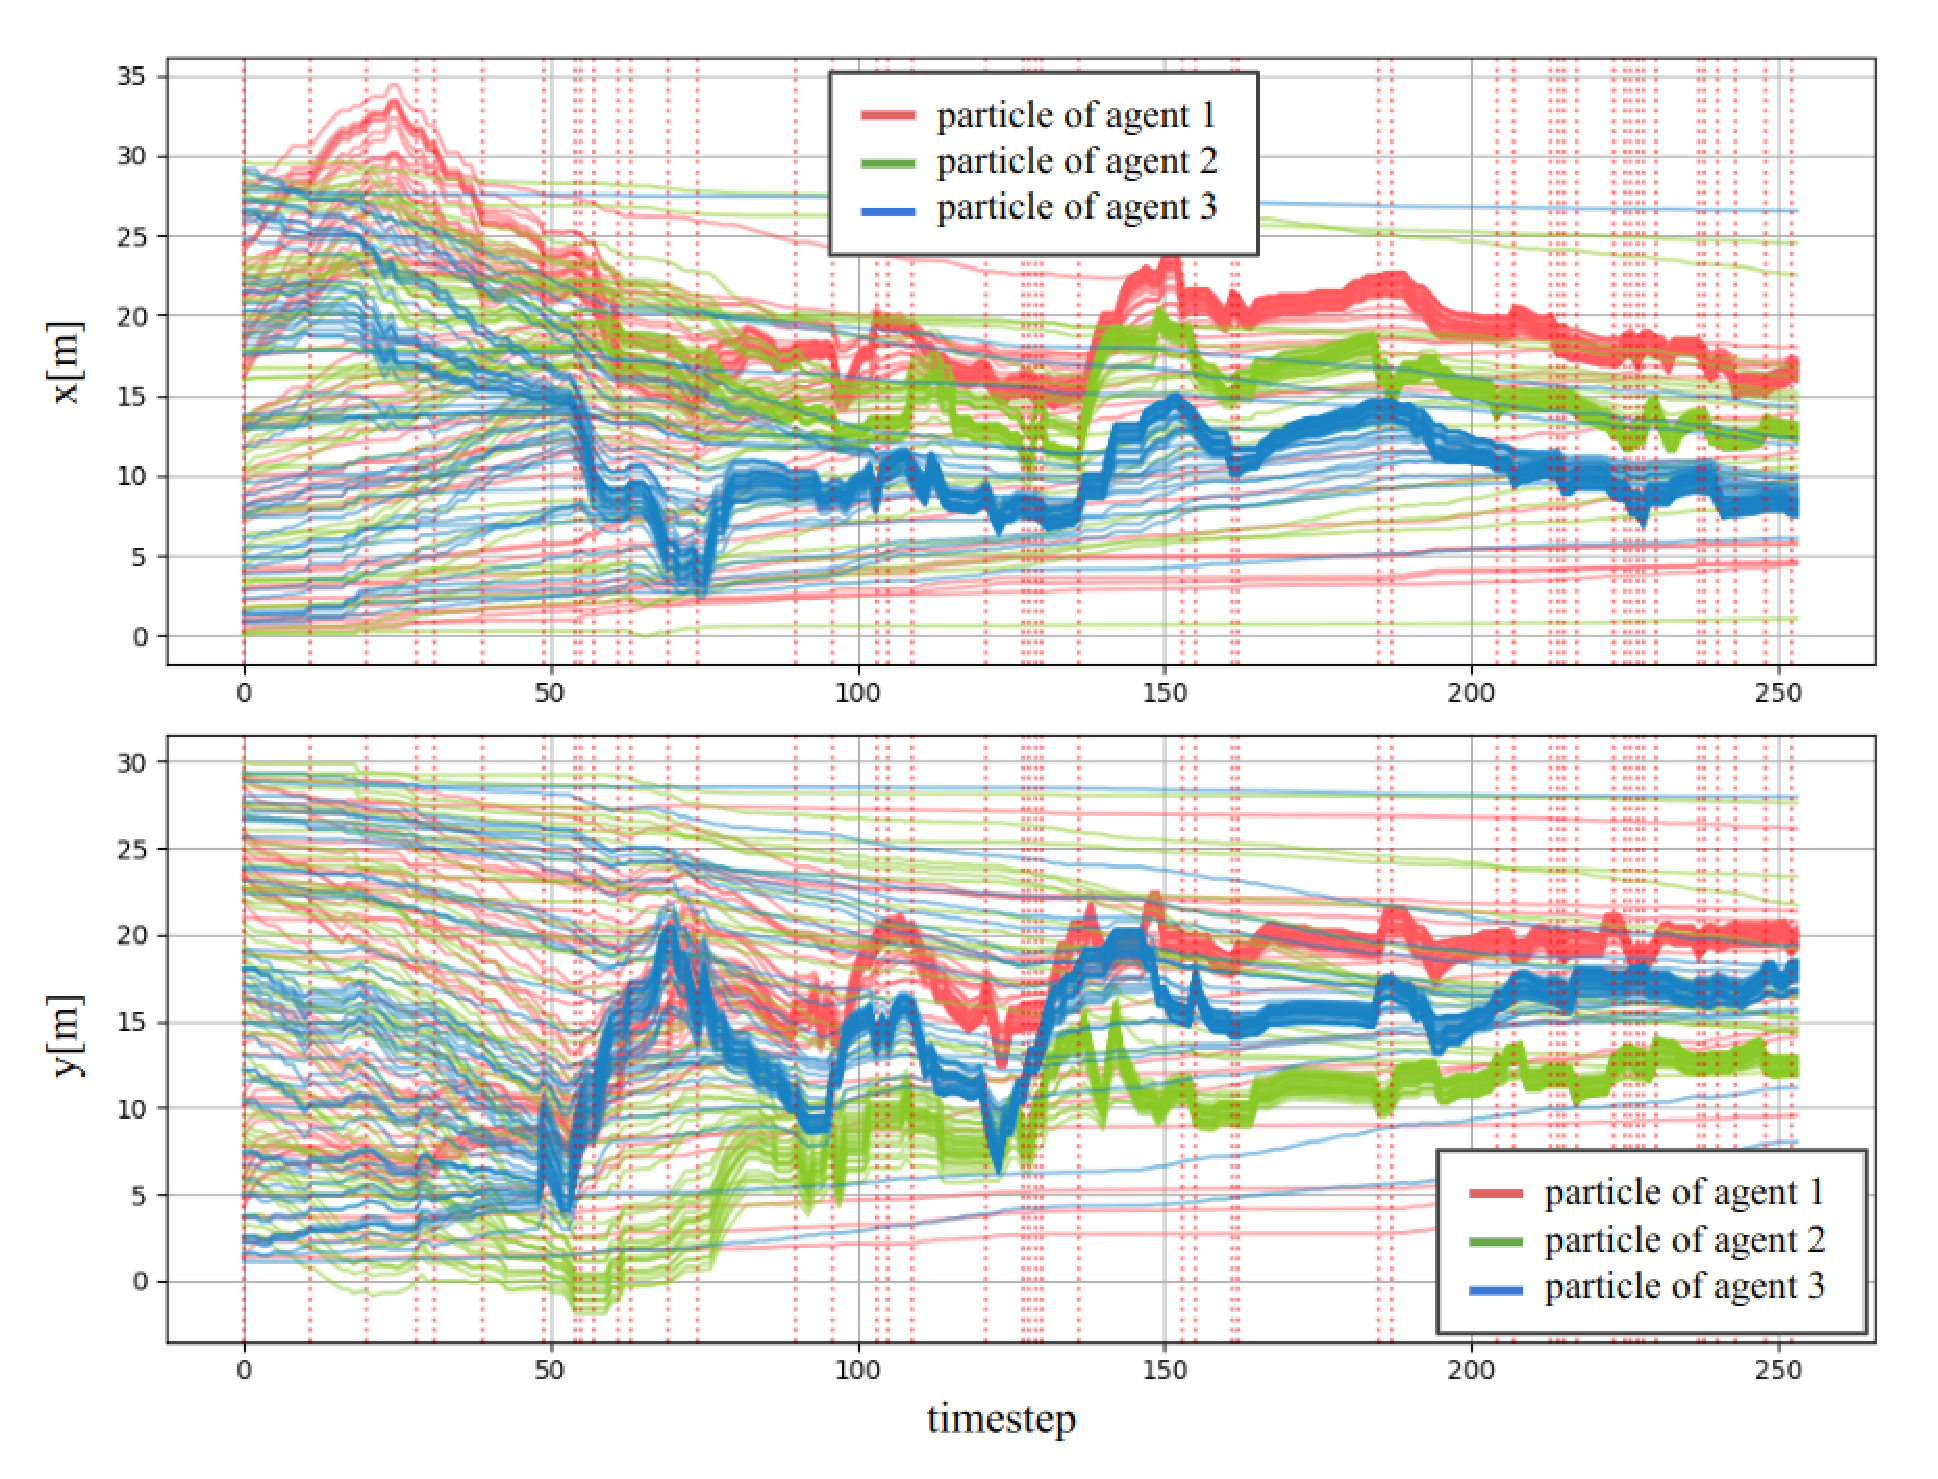
\includegraphics[width=\linewidth]{Fig/2d_plot.eps}
		\caption{2次元の協調自己位置推定シミュレーションにおける全パーティクルの座標$p_{i,r}$の時間遷移をx座標及びy座標で分けて示したもの.
    プロットされた各線はそれぞれエージェントのパーティクルの座標を示す.
    赤色の縦点線は外れ値が生成されたステップを示す.}
		\label{fig:plot_1}
	\end{center}
	\vspace{-2mm}
\end{figure}

\subsection{Three-dimensional case}

SE(3)における提案手法の検証として,3Dにおける協調自己位置推定シナリオのシミュレーションを行った.
3次元空間での検証は,実際のUAVの運用環境により近い状況を再現するために重要である.
特に,回転行列を含む特殊ユークリッド群SE(3)上での状態推定は,姿勢と位置の両方を同時に扱う必要があり,計算的にも理論的にも2次元の場合よりも複雑である.
シミュレーション条件を表\ref{tb:sim2}に示す.

\begin{table}[h]
\caption{シミュレーション条件}
  \centering
  \begin{tabular}{l|c} \hline
    項目 & 値  \\ \hline
    エージェント数 & 3  \\
    エージェントごとのパーティクル数 & 50  \\ 
    時間ステップ数 & 250 \\
    総マッチング数 & 250 \\ 
    誤マッチング数 & 48 \\
    外れ値の割合 & $\simeq$ 0.2 \\ \hline
  \end{tabular}
  \label{tb:sim2}
\end{table}

シミュレーションの設定は,2Dと同様に真のエージェント位置を仮定し,毎ステップランダムなエージェントペアの相対値が得られるという前提のもと,一定の割合で外れ値が混入する環境を再現するものである.
3dシミュレーションにおいては真のエージェント位置をそれぞれ
\begin{equation}
  \begin{aligned}
  x_i = 
  \begin{pmatrix}
    {\mathbf{I}} & {\mathbf{t}}_i \\
    {\mathbf{0}}^T & 1
  \end{pmatrix}, {\mathbf{t}}_1 = \begin{bmatrix} 0 \\ 0 \\ 0 \end{bmatrix}, {\mathbf{t}}_2 = \begin{bmatrix} 2 \\ 0 \\ 0 \end{bmatrix}, {\mathbf{t}}_3 = \begin{bmatrix} 0 \\ 2 \\ 0 \end{bmatrix}
  \end{aligned}
\end{equation}
として,推定を行った.

3次元シミュレーションでは,Fig. \ref{fig:3d_simulation}に示すとおり2次元の場合と同様に,各エージェントが初期状態から徐々に正確な位置・姿勢推定に収束する過程を観察した.特に注目すべき点として,SE(3)上での勾配計算が正確に機能し,回転成分と並進成分の両方において適切な収束が見られた.また,外れ値が存在する環境下でも,提案手法のADMMによる合意アルゴリズムが効果的に機能し,全エージェントが一貫した状態推定に収束することが確認された.

2次元の場合と比較して,3次元シミュレーションでは計算コストが増加するものの,GPUによる並列処理の恩恵により,実用的な計算時間内で結果を得ることができた.

\begin{figure}[t]
	\begin{center}
		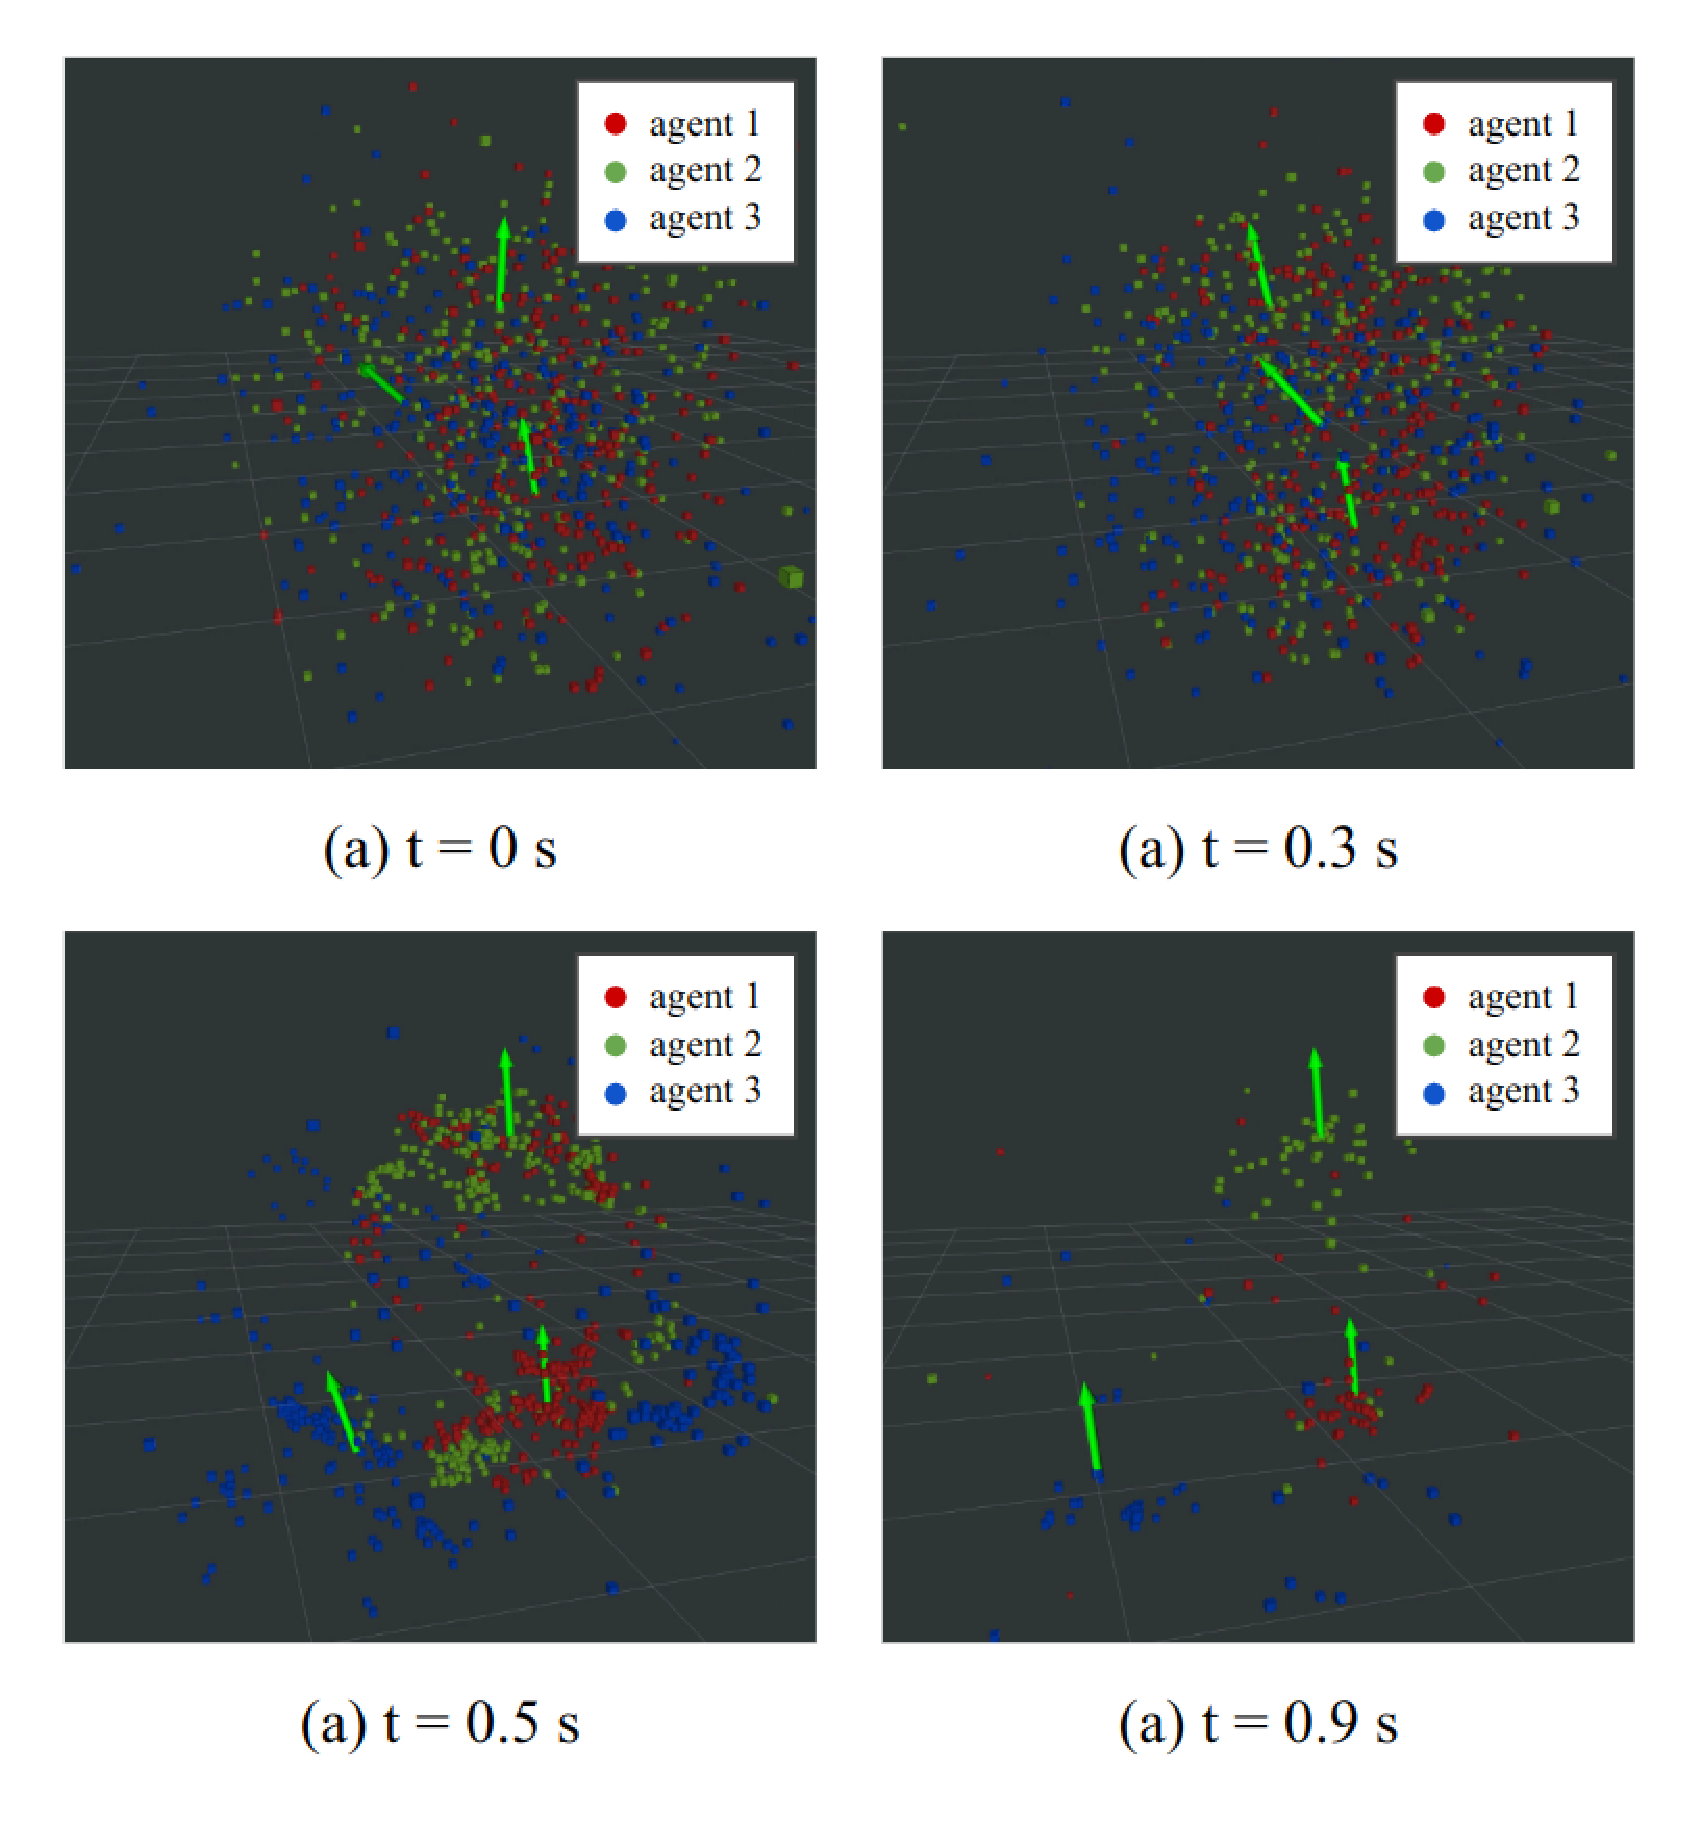
\includegraphics[width=\linewidth]{Fig/3d_simulation.eps}
		\caption{外れ値の割合が0.2の場合における,
    3次元の協調自己位置推定シミュレーション.画像はそれぞれシミュレーション開始から(a)0s, (b)0.3s, (c)0.5s, (d)0.9s経過した様子である.
    点群は各エージェントのパーティクルの座標$p_{i,r}$である.黄緑色の矢印は各エージェントの点群から推定した自己位置である.}
		\label{fig:3d_simulation}
	\end{center}
	\vspace{-2mm}
\end{figure}

\section{Extension to the Visual Inertial System}

提案手法を現実の協調自己位置推定システムに適用するための部分的な検証として,BMI270 IMUとIntel RealSense D435カメラを搭載したUAVを用いた単機での実機実験を行った.
実機実験は,シミュレーションでは再現が困難な実世界の複雑な要素(センサノイズ,環境の不確実性,計算遅延など)を考慮するために不可欠である.特に,Visual-Inertial Systemにおいては,カメラとIMUの統合による自己位置推定の精度と安定性を実環境で検証することが重要となる.

予測ステップでは,式(\ref{eq:map})の$P(x_{t+1}|z_t)$を計算する必要がある.これは$t$ステップまでの情報から$t+1$ステップの状態を予測する操作であり,VINSでは次のようにIMUから得られる加速度$a_m$,角速度$\omega_m$を数値積分することで得られる.SE(3)上での数値積分は文献\cite{Forster2017}などと類似した枠組みを用いて

\begin{equation}
\begin{aligned}\label{eq:predict}
p_{k+1} &=p_{k} + v_{k}\Delta t \\
&\quad+ \int\!\!\!\int_{t\in [t_k,t_{k+1}]} \underbrace{\left \{ R_{k}(a_m-b_a-\eta_{ad})+g\right \}}_{\hat a}dt^2,\\
v_{k+1} &=v_{k} + \int_{t\in [t_k,t_{k+1}]} \hat a dt,\\
R_{k+1} &=R_{k} \otimes \exp \left( \int_{t\in [t_k,t_{k+1}]} \underbrace{(\omega_m-b_g-\eta_{gd})}_{\hat \omega} dt \right),
\end{aligned}
\end{equation}

のように計算できる.ここで,$p$は位置,$v$は速度,$R$は姿勢を表す回転行列,$b_a, b_g$はそれぞれ加速度,角速度のバイアス, $\eta_{ad}, \eta_{gd}$は白色ノイズである.
数値積分によって得られた変換$T_{t\rightarrow t+1}\in \text{SE}(3)$によって各パーティクルは

\begin{equation}
\begin{aligned}\label{eq:step}
\hat x_{t+1}^i = x_{t}^i T_{t\rightarrow t+1}, \forall i,
\end{aligned}
\end{equation}

のように更新される.

本実験では,特に以下の点に焦点を当てて検証を行った:
\begin{itemize}
\item 実環境における外れ値(誤ったビジュアルマッチング)に対するロバスト性
\item IMUの積分誤差の蓄積に対する補正能力
\item 多峰性分布の表現による不確実性の適切な取り扱い
\item リアルタイム処理の実現可能性
\end{itemize}

行った実機実験の条件を表\ref{tb:sim3}に示す.

\begin{table}[h]
\caption{実機実験条件}
  \centering
  \begin{tabular}{l|c} \hline
    項目 & 値  \\ \hline
    エージェント数 & 1  \\
    パーティクル数 & 20 /agent  \\
    外れ値の割合 & 〜10\% \\
    Ground Truth & OptiTrack Flex13, Naturalpoint \\ \hline
  \end{tabular}
  \label{tb:sim3}
\end{table}

この実験では,6DoF状態推定においてSVGDに基づくSPFが誤差蓄積を低減し,ベンチマーク手法(D2SLAM等)と比較して精度向上している様子が見られた.特に,長時間の運用において従来手法では徐々に増加する位置誤差が,提案手法では効果的に抑制されることが確認された.これは,パーティクルの多様性を維持しながら勾配情報を活用することで,局所的な最適解に陥ることなく,より正確な状態推定が可能になったためと考えられる.

複数機での完全な協調効果は未検証であるが,本研究で提案するSPFベースのフレームワークが実環境下でも有用である可能性を示す初期的結果が得られた.単機での実験結果は,複数機への拡張における基礎的な性能指標として重要であり,特に計算効率とロバスト性の観点から,提案手法の実用性を示唆している.

Fig. \ref{fig:ros_demo}はROSを用いて自己位置推定を行った様子である.
Fig. \ref{fig:benchmark}は各パーティクルとベンチマーク手法におけるGround Truthとの誤差遷移を示している.ここから,時系列の大部分で提案手法がベンチマーク手法より高精度に推定できていることが確認できる.本実験によって6 DoFにおけるパーティクルの勾配更新法の有効性が検証できたが,今後の研究としては複数機を用いた合意手法の検証を行いたい.

\begin{figure}[t]
	\begin{center}
		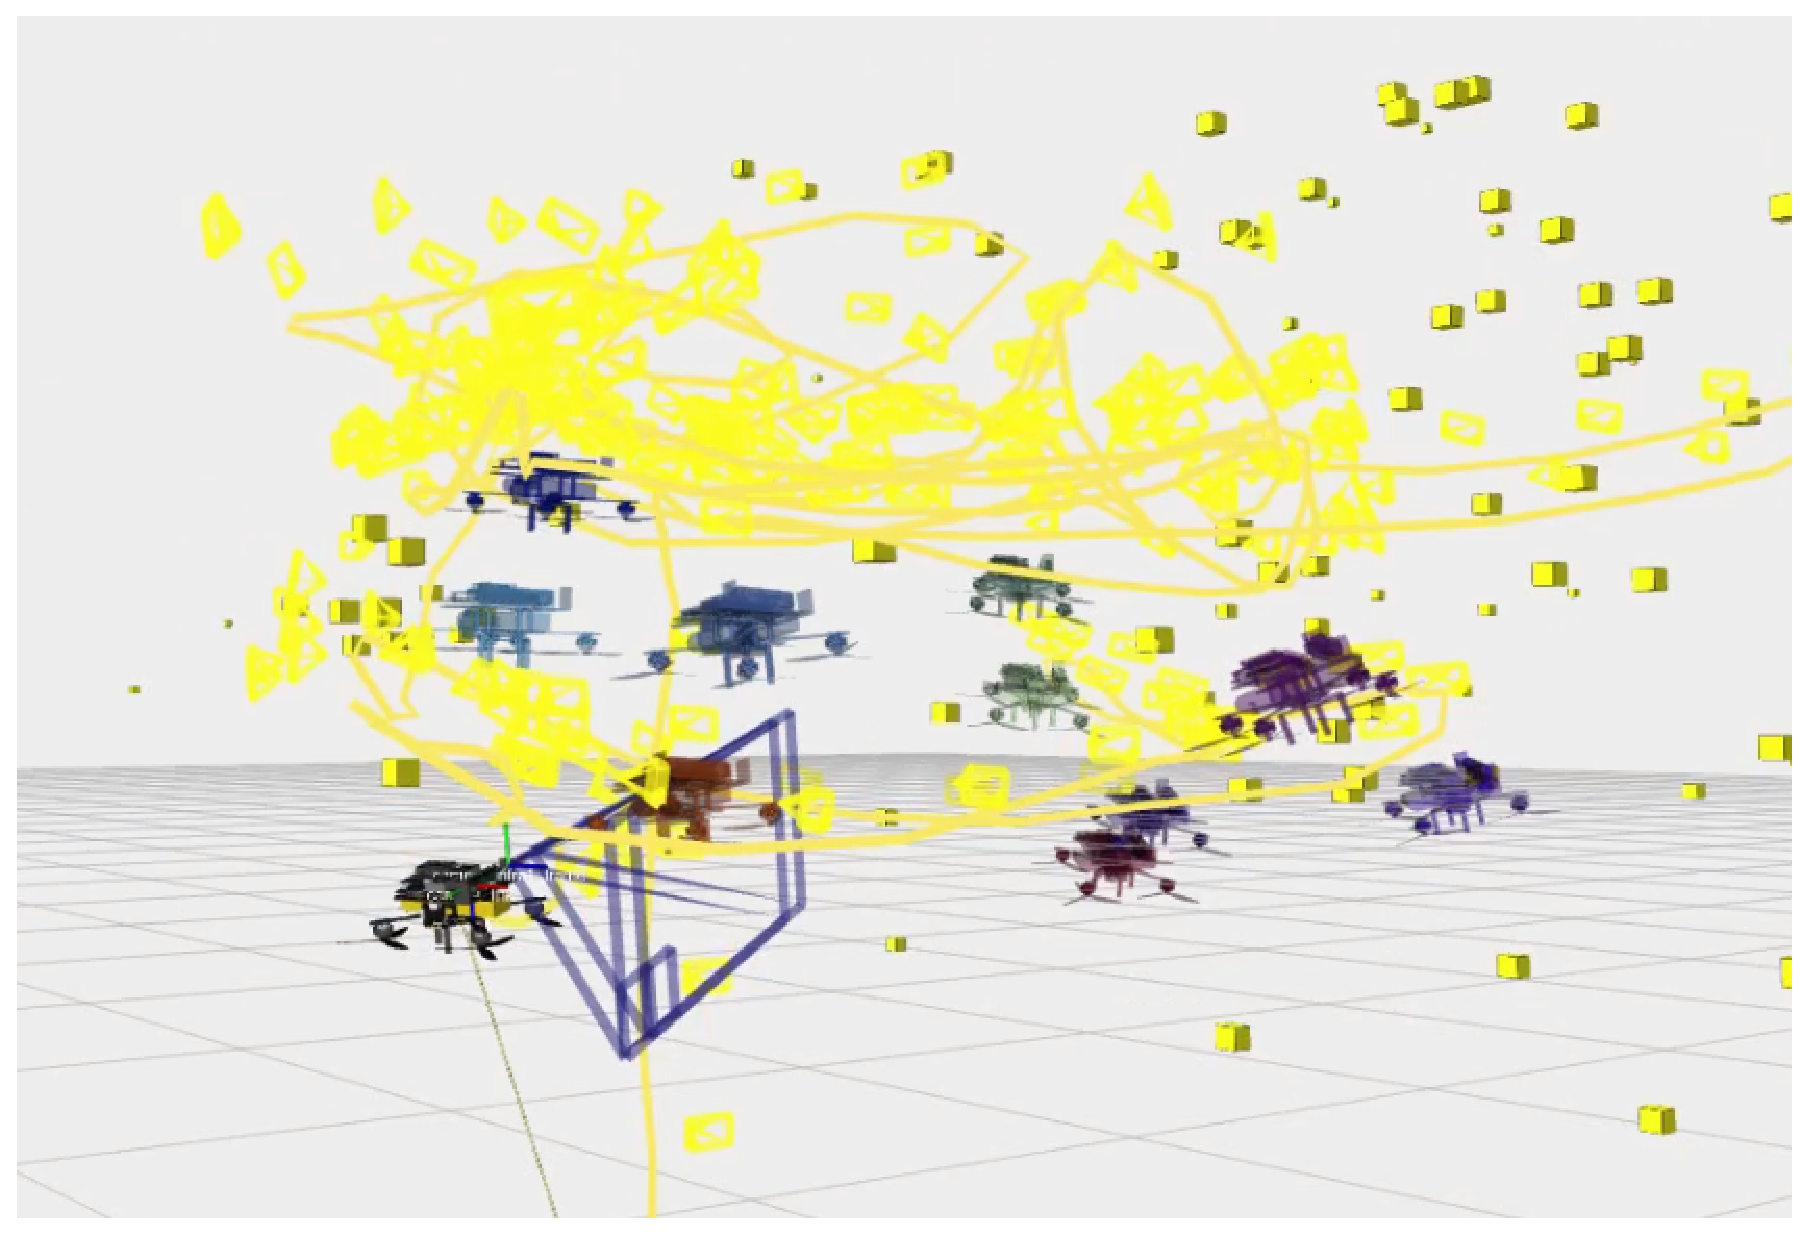
\includegraphics[width=\linewidth]{Fig/particle_filter_demo.eps}
		\caption{ROS上での提案アルゴリズムの検証の様子.薄いドローンの3dモデルがパーティクルの座標$p_{i,r}$,濃い3Dモデルがエージェントの推定位置である.黄色の点群はsuperpointにより抽出した特徴点,黄色線はエージェントの推定軌道である.}
		\label{fig:ros_demo}
	\end{center}
	\vspace{-2mm}
\end{figure}

\begin{figure}[t]
	\begin{center}
		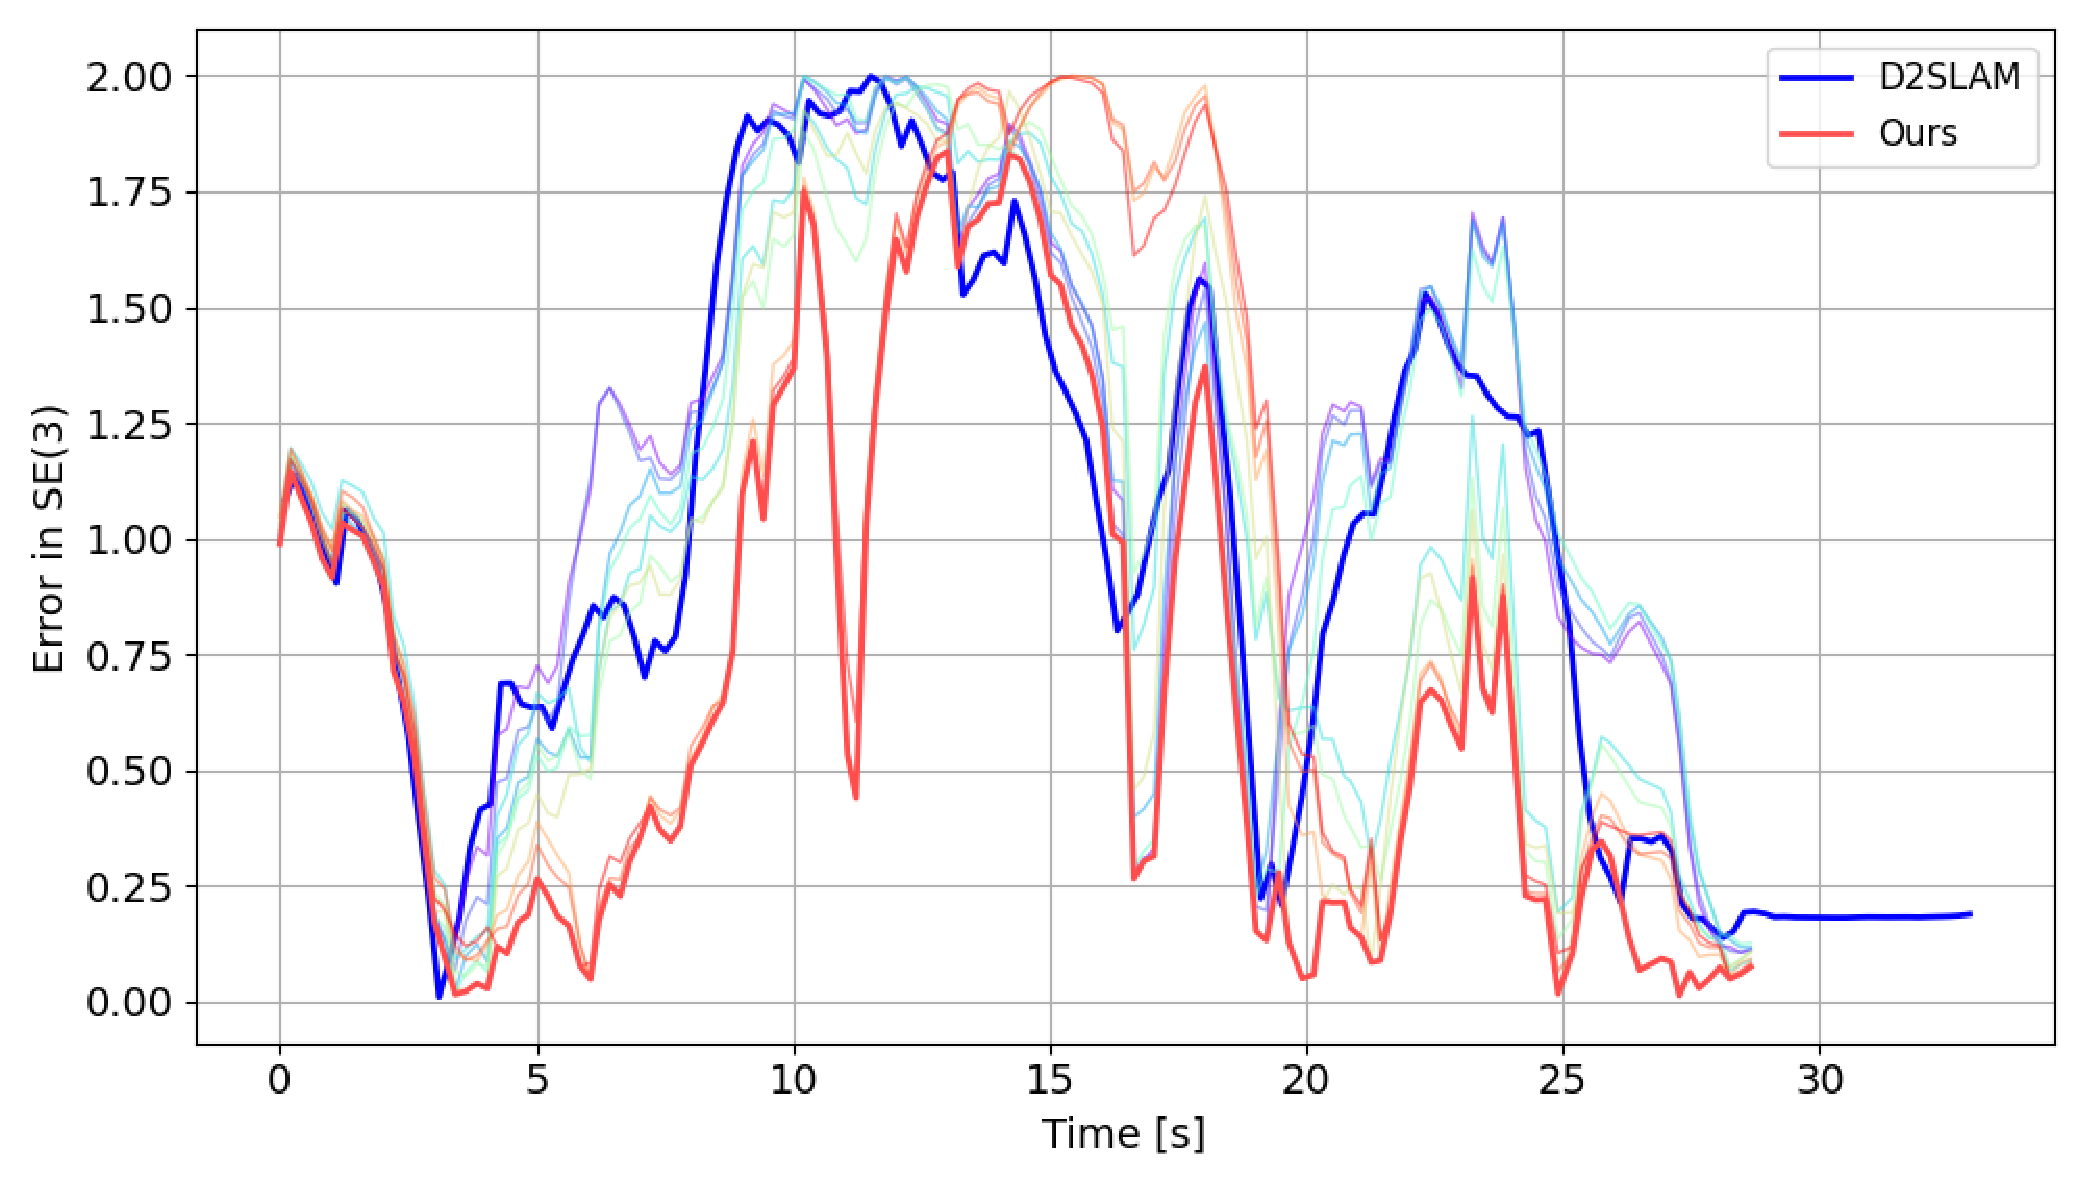
\includegraphics[width=\linewidth]{Fig/benchmark.eps}
		\caption{ROS上で検証した提案手法とD2SLAMのベンチマーク.薄い線は各パーティクルにおけるGround Truthとの誤差時間遷移,オレンジの濃い線は提案手法の推定状態における誤差時間遷移である.濃い青線はD2SLAMの誤差遷移である.}
		\label{fig:benchmark}
	\end{center}
	\vspace{-2mm}
\end{figure}

\section{Conclusion}

本稿では,SPFとRelaxed ADMMを組み合わせた新たなフレームワークを提案し,単調な広域環境におけるUAVの協調自己位置推定問題に取り組んだ.
特に,従来の協調自己位置推定手法が直面していた「外れ値の影響」と「エージェント間の一貫した状態推定」という2つの根本的な課題に対して,理論的に整合性のある解決策を提示した.

提案手法は,複数エージェント間の合意制約と多峰性分布の扱いを同時に可能にし,従来手法では困難であった外れ値混在環境下での安定的な位置合意を実現する.
具体的には,以下の3つの技術的貢献により,これを達成した:(1) 特殊ユークリッド空間SE(d)上での確率分布の表現と操作,(2) ADMMによる分散最適化フレームワークの導入,(3) パーティクルベースの表現による不確実性の適切な取り扱い.これらの組み合わせにより,単調環境における協調自己位置推定の精度と安定性を大幅に向上させることができた.

シミュレーションおよび実機実験(単機)結果から,SPFを用いることによって,分布近似と勾配情報を活用し,既存手法よりもロバストかつ柔軟な自己位置推定が可能であることが示唆された.
特に,外れ値の割合が0.2程度の環境下でも安定した収束が得られたことは,実用的な観点から重要な成果である.また,GPUを活用した並列計算により,計算コストの増加を抑えつつ,リアルタイム処理を実現できることも確認された.

今後は,複数UAVによる実機レベルの大規模実験を通じて,提案手法の有効性とスケーラビリティをさらに検証していく予定である.

\appendix
\section{定理の証明}

\subsection{定理2(確率分布に対するRelaxed ADMMアルゴリズム)の証明}
本証明では,式(\ref{eq:kl_consensus_relaxed})で表される確率分布に対する制約付き最適化問題を解くためのRelaxed ADMMアルゴリズムの導出過程を示す.まず,標準的なRelaxed ADMMの枠組みを確率分布の最適化問題に適用し,その後,確率分布特有の性質を考慮した変形を行う.

まず,スラック変数$y_{ij}$を導入した問題(\ref{eq:kl_consensus_relaxed})に対して,拡張ラグランジアンを構築する.エージェント$i$とエージェント$j$の間の制約に関する拡張ラグランジアンは以下のように表される:

\begin{equation}
\begin{aligned}
y^+_{ij}&= \underset{y_{ij}}{\text{arg min}}\: {\mathcal{L}}_{g,\gamma}(z_{ij,i} + z_{ij,j})\\
&=  \underset{y_{ij}}{\text{arg min}}\: \langle z_{ij,i} + z_{ij,j}, y_{ij} \rangle +  \frac \gamma 2\|y_{ij}\|^2 ,
\end{aligned}
\end{equation}

ここで,$z_{ij,i}$と$z_{ij,j}$はそれぞれエージェント$i$と$j$のラグランジュ乗数,$\gamma$はペナルティパラメータである.この最小化問題を解くと,$y_{ij}$の更新式が得られる.次に,補助変数$\omega_g$を以下のように計算する:

\begin{equation}
\begin{aligned}
(\omega_g)_{ij,i} &= z_{ij,i} - \gamma y^+_{ij},
\end{aligned}
\end{equation}

この補助変数を用いて,エージェント$i$の状態$x_i$の更新を行う.確率分布$P_i$に対する拡張ラグランジアンは以下のように表される:

\begin{equation}
\begin{aligned}
x^+_i&= \underset{x_i}{\text{arg min}}\: {\mathcal{L}}_{F,\gamma}(x_i, z_i)\\
&=  \underset{x_i}{\text{arg min}}\: D_{KL} ({P_i}_{[T]}\|{P_Q}_i) \\
& \quad - \sum_{j\in {\mathcal{E}}_i} \int_{P_i} \left\{2(\omega_g)_{ij,i} - z_{ij,i}\right\} dx_i\\
& \quad + \frac{\gamma}{2}|{\mathcal{E}}_i|\int_{P_i} dx_i^2,
\end{aligned}
\end{equation}

ここで,$D_{KL} ({P_i}_{[T]}\|{P_Q}_i)$はKLダイバージェンス項,${\mathcal{E}}_i$はエージェント$i$の隣接エージェント集合である.この最小化問題を解くことで,確率分布$P_i$の更新が行われる.

次に,もう一つの補助変数$\omega_f$を計算する:

\begin{equation}
\begin{aligned}
(\omega_f)_{ij,i} &= 2(\omega_g)_{ij,i} - z_{ij,i} - \gamma x^+_{i},
\end{aligned}
\end{equation}

最後に,ラグランジュ乗数$z_{ij,i}$を更新する:

\begin{equation}
\begin{aligned}
z^+_{ij,i}&=z_{ij,i}+\eta((\omega_f)_{ij,i}-(\omega_g)_{ij,i}),
\end{aligned}
\end{equation}

ここで,$\eta$はステップサイズパラメータである.

これらの更新式を整理すると,定理2で示したRelaxed ADMMアルゴリズムが得られる.このアルゴリズムは,各エージェントの局所的な確率分布の更新と,エージェント間の合意制約の両方を同時に最適化することができる.特に,確率分布の期待値表現を用いることで,式(\ref{eq:prob_relaxed_admm})に示した形式に変換できる.

\subsection{定理3(指数的なペナルティとしての追加項)の証明}
本証明では,確率分布に対する最適化問題において,追加のペナルティ項が基準分布に対してどのように作用するかを示す.具体的には,KLダイバージェンスと追加項を含む最適化問題の解が,基準分布に対して指数的な重みを掛けた形で表現できることを証明する.

まず,目的関数を $P_i$ について書き下すと,
\begin{equation}
\begin{aligned}
{\mathcal{J}}(P_i) &= \int P_i(x_i)\log\frac{P_i(x_i)}{P_{Q_i}(x_i)}\,dx_i \\
&+ \sum_{r \in {\mathcal{E}}_i}\int P_i(x_i) z_{ir,r}(x_i)\,dx_i  \\
&+ \frac{\gamma}{2}|{\mathcal{E}}_i| \int P_i(x_i) x_i^2\, dx_i,
\end{aligned}
\end{equation}

ここで,第1項はKLダイバージェンス$D_{KL}(P_i \,\|\, P_{Q_i})$,第2項と第3項は追加のペナルティ項である.これらの項を一つの積分にまとめると,

\begin{equation}
\begin{aligned}
{\mathcal{J}}(P_i) &= \int P_i(x_i)\biggl(\log P_i(x_i) - \log P_{Q_i}(x_i) \\
&\quad + \sum_{r \in {\mathcal{E}}_i} z_{ir,r}(x_i)
+ \frac{\gamma}{2}|{\mathcal{E}}_i| x_i^2 \biggr) dx_i,
\end{aligned}
\end{equation}

次に,$P_i$ に対して最適化を行う.ただし,$P_i$は確率分布であるため,$\int P_i(x_i)\,dx_i=1$ という制約がある.この制約付き最適化問題を解くために,ラグランジュ乗数法を用いる.ラグランジュ乗数 $\lambda$ を導入すると,

\begin{equation}
\begin{aligned}
&\delta_{P_i}\Bigl[\int P_i(x_i)\log P_i(x_i)\,dx_i\\
&- \int P_i(x_i)\log P_{Q_i}(x_i)\,dx_i\\
&+ \int P_i(x_i)\bigl(\sum_{r \in {\mathcal{E}}_i} z_{ir,r}(x_i)+ \frac{\gamma}{2}|{\mathcal{E}}_i|x_i^2\bigr)dx_i\\
&- \lambda \left(\int P_i(x_i)\,dx_i -1\right)\Bigr]= 0,
\end{aligned}
\end{equation}

ここで,$\delta_{P_i}$は$P_i$に関する変分微分を表す.この変分微分を計算すると,

\begin{equation}
\begin{aligned}
&\log P_i(x_i) + 1 - \log P_{Q_i}(x_i) \\
&+ \sum_{r \in {\mathcal{E}}_i} z_{ir,r}(x_i) 
+ \frac{\gamma}{2}|{\mathcal{E}}_i| x_i^2 - \lambda = 0,
\end{aligned}
\end{equation}

この式を$P_i(x_i)$について解くと,

\begin{equation}
\begin{aligned}
&\log P_i(x_i) = \log P_{Q_i}(x_i) \\
&- \sum_{r \in {\mathcal{E}}_i} z_{ir,r}(x_i)
- \frac{\gamma}{2}|{\mathcal{E}}_i| x_i^2 + \lambda - 1,
\end{aligned}
\end{equation}

ここで,$\lambda-1$は定数であり,確率分布の正規化条件を満たすための値である.これを$-\log Z$と置くと,

\begin{equation}
\begin{aligned}
&\log P_i(x_i) = \log P_{Q_i}(x_i) \\
&- \sum_{r \in {\mathcal{E}}_i} z_{ir,r}(x_i)
- \frac{\gamma}{2}|{\mathcal{E}}_i| x_i^2 - \log Z,
\end{aligned}
\end{equation}

両辺の指数をとると,最適分布$P_i^*(x_i)$は次のように表される:

\begin{equation}
\begin{aligned}
P_i^*(x_i) = \frac{P_{Q_i}(x_i)\exp\left(- \sum_{r \in {\mathcal{E}}_i} z_{ir,r}(x_i) 
- \frac{\gamma}{2}|{\mathcal{E}}_i| x_i^2\right)}{Z},
\end{aligned}
\end{equation}

ここで,$Z$は正規化定数であり,

\begin{equation}
\begin{aligned}
Z = \int P_{Q_i}(x_i)\exp\left(- \sum_{r \in {\mathcal{E}}_i} z_{ir,r}(x_i) 
- \frac{\gamma}{2}|{\mathcal{E}}_i| x_i^2\right) dx_i,
\end{aligned}
\end{equation}

と表される.この結果から,追加のペナルティ項

\begin{equation}
\begin{aligned}
\sum_{r \in {\mathcal{E}}_i} z_{ir,r}(x_i) \;+\; \frac{\gamma}{2}|{\mathcal{E}}_i|x_i^2,
\end{aligned}
\end{equation}

は,基準分布$P_{Q_i}(x_i)$に対して指数関数の形で重みを与えることがわかる.すなわち,これらの項は基準分布に対して指数的なペナルティとして作用し,最適分布の形状を特徴づける重要な役割を果たしている.

以上により,定理3が証明された.

\begin{thebibliography}{99}
\bibitem{Qin2018} T. Qin, P. Li, and S. Shen, ``VINS-Mono: A Robust and Versatile Monocular Visual-Inertial State Estimator,'' {\it IEEE Transactions on Robotics}, Vol. 34, No. 4, pp. 1004-1020, 2018.

\bibitem{Chen2021} C. Chen, H. Zhu, M. Li, and S. You, ``A Review of Visual-Inertial Simultaneous Localization and Mapping from Filtering-Based and Optimization-Based Perspectives,'' {\it Robotics}, Vol. 7, No. 3, pp. 45, 2021.

\bibitem{Zhou2018} X. Zhou, J. Zhu, H. Zhou, C. Xu, and F. Gao, ``EGO-Swarm: A Fully Autonomous and Decentralized Quadrotor Swarm System in Cluttered Environments,'' {\it IEEE International Conference on Robotics and Automation (ICRA)}, pp. 7308-7315, 2018.

\bibitem{Liu2016} Q. Liu and D. Wang, ``Stein Variational Gradient Descent: A General Purpose Bayesian Inference Algorithm,'' {\it Advances in Neural Information Processing Systems (NeurIPS)}, pp. 2378-2386, 2016.

\bibitem{Koide2021} K. Koide, J. Miura, and E. Menegatti, ``A Portable 3D LIDAR-based System for Long-term and Wide-area People Behavior Measurement,'' {\it International Journal of Advanced Robotic Systems}, Vol. 16, No. 2, pp. 1-15, 2021.

\bibitem{Bloesch2017} M. Bloesch, S. Omari, M. Hutter, and R. Siegwart, ``Robust Visual Inertial Odometry Using a Direct EKF-Based Approach,'' {\it IEEE/RSJ International Conference on Intelligent Robots and Systems (IROS)}, pp. 298-304, 2017.

\bibitem{Forster2017} C. Forster, L. Carlone, F. Dellaert, and D. Scaramuzza, ``On-Manifold Preintegration for Real-Time Visual-Inertial Odometry,'' {\it IEEE Transactions on Robotics}, Vol. 33, No. 1, pp. 1-21, 2017.

\bibitem{Xu2020} W. Xu, F. Gao, and S. Shen, ``D2SLAM: Decentralized and Distributed Collaborative Visual-Inertial SLAM System for Aerial Swarm,'' {\it IEEE Transactions on Robotics}, Vol. 36, No. 6, pp. 1864-1879, 2020.

\bibitem{Maken2021} F. P. Maken, F. Ramos, and L. Ott, ``Stein Particle Filter: A Stein Variational Gradient Descent Approach to Sequential Inference,'' {\it IEEE International Conference on Robotics and Automation (ICRA)}, pp. 14591-14597, 2021.

\bibitem{Schmuck2018} P. Schmuck and M. Chli, ``CCM-SLAM: Robust and Efficient Centralized Collaborative Monocular Simultaneous Localization and Mapping for Robotic Teams,'' {\it Journal of Field Robotics}, Vol. 36, No. 4, pp. 763-781, 2018.

\bibitem{Bastianello2020} N. Bastianello, R. Carli, L. Schenato, and M. Todescato, ``Asynchronous Distributed Optimization over Lossy Networks via Relaxed ADMM: Stability and Linear Convergence,'' {\it IEEE Transactions on Automatic Control}, Vol. 65, No. 8, pp. 3350-3365, 2020.

\bibitem{Arandjelovic2016} R. Arandjelovic, P. Gronat, A. Torii, T. Pajdla, and J. Sivic, ``NetVLAD: CNN Architecture for Weakly Supervised Place Recognition,'' {\it IEEE Conference on Computer Vision and Pattern Recognition (CVPR)}, pp. 5297-5307, 2016.

\bibitem{DeTone2018} D. DeTone, T. Malisiewicz, and A. Rabinovich, ``SuperPoint: Self-Supervised Interest Point Detection and Description,'' {\it IEEE/CVF Conference on Computer Vision and Pattern Recognition Workshops (CVPRW)}, pp. 337-349, 2018.

\bibitem{Peng2016} Z. Peng, Y. Xu, M. Yan, and W. Yin, ``ARock: An Algorithmic Framework for Asynchronous Parallel Coordinate Updates,'' {\it SIAM Journal on Scientific Computing}, Vol. 38, No. 5, pp. A2851-A2879, 2016.

\bibitem{Boyd2011} S. Boyd, N. Parikh, E. Chu, B. Pelegris, and J. Eckstein, ``Distributed Optimization and Statistical Learning via the Alternating Direction Method of Multipliers,'' {\it Foundations and Trends in Machine Learning}, Vol. 3, No. 1, pp. 1-122, 2011.

\end{thebibliography}

\end{document}
